\documentclass[a4paper,11pt,fleqn,dvipsnames,twoside,openany]{memoir} 	% Openright aabner kapitler paa hoejresider (openany begge)

%%%% PACKAGES %%%%

% ¤¤ Oversaettelse og tegnsaetning ¤¤ %
\usepackage[utf8]{inputenc}					% Input-indkodning af tegnsaet (UTF8)
\usepackage[english]{babel}					% Dokumentets sprog
\usepackage[T1]{fontenc}					% Output-indkodning af tegnsaet (T1)
\usepackage{ragged2e,anyfontsize}			% Justering af elementer
\usepackage{fixltx2e}						% Retter forskellige fejl i LaTeX-kernen
																			
% ¤¤ Figurer og tabeller (floats) ¤¤ %
\usepackage{changepage}						% http://ctan.org/pkg/changepage
\usepackage{mathtools}
\DeclarePairedDelimiter\ceil{\lceil}{\rceil}
\DeclarePairedDelimiter\floor{\lfloor}{\rfloor}

\addtolength{\jot}{2ex}

\usepackage{graphicx}						% Haandtering af eksterne billeder (JPG, PNG, EPS, PDF)
\usepackage{caption}
\usepackage{subcaption} 						
%\usepackage{eso-pic}						% Tilfoej billedekommandoer paa hver side
%\usepackage{wrapfig}						% Indsaettelse af figurer omsvoebt af tekst. \begin{wrapfigure}{Placering}{Stoerrelse}
\usepackage{multirow}                		% Fletning af raekker og kolonner (\multicolumn og \multirow)
\usepackage{multicol}         	        	% Muliggoer output i spalter
\usepackage{rotating}						% Rotation af tekst med \begin{sideways}...\end{sideways}
\usepackage{colortbl} 						% Farver i tabeller (fx \columncolor og \rowcolor)
\usepackage[table]{xcolor}				 	% Definer farver med \definecolor. Se mere: http://en.wikibooks.org/wiki/LaTeX/Colors
\usepackage{flafter}						% Soerger for at floats ikke optraeder i teksten foer deres reference
\let\newfloat\relax 						% Justering mellem float-pakken og memoir
\usepackage{float}							% Muliggoer eksakt placering af floats, f.eks. \begin{figure}[H]
\usepackage{wrapfig}

% ¤¤ Matematik mm. ¤¤
\usepackage{amsmath,amssymb,stmaryrd} 		% Avancerede matematik-udvidelser
\usepackage{textcomp}                 		% Symbol-udvidelser (f.eks. promille-tegn med \textperthousand )
\usepackage{rsphrase}						% Kemi-pakke til RS-saetninger, f.eks. \rsphrase{R1}

% ¤¤ Referencer og kilder ¤¤ %
\usepackage[danish]{varioref}				% Muliggoer bl.a. krydshenvisninger med sidetal (\vref)
\usepackage[square,sort,comma,numbers]{natbib}							% Udvidelse med naturvidenskabelige citationsmodeller
%\usepackage{xr}							% Referencer til eksternt dokument med \externaldocument{<NAVN>}
%\usepackage{glossaries}					% Terminologi- eller symbolliste (se mere i Daleifs Latex-bog)

% ¤¤ Misc. ¤¤ %
\usepackage{lipsum}							% Dummy text \lipsum[..]
\usepackage[shortlabels]{enumitem}			% Muliggoer enkelt konfiguration af lister
\usepackage{pdfpages}						% Goer det muligt at inkludere pdf-dokumenter med kommandoen \includepdf[pages={x-y}]{fil.pdf}	
\pdfoptionpdfminorversion=6					% Muliggoer inkludering af pdf dokumenter, af version 1.6 og hoejere
\pretolerance=2500 							% Justering af afstand mellem ord (hoejt tal, mindre orddeling og mere luft mellem ord)

% Kommentarer og rettelser med \fxnote. Med 'final' i stedet for 'draft' udloeser hver note en error i den faerdige rapport.
\usepackage[footnote,final,english,silent,nomargin]{fixme}		
\usepackage[bottom]{footmisc}

\fxsetup{
    status=draft,
    author=,
    layout=inline,
    theme=color
}

\definecolor{fxnote}{rgb}{0.8000,0.0000,0.0000}
% define the background colour:
\colorlet{fxnotebg}{yellow}

% refedine the layout macro:
\makeatletter
\renewcommand*\FXLayoutInline[3]{%
  \@fxdocolon {#3}{%
    \@fxuseface {inline}%
    \colorbox{fx#1bg}{\color {fx#1}\ignorespaces #3\@fxcolon #2}}}
\makeatother


%%%% CUSTOM SETTINGS %%%%

% ¤¤ Marginer ¤¤ %
\setlrmarginsandblock{2.5cm}{2.5cm}{*}		% \setlrmarginsandblock{Indbinding}{Kant}{Ratio}
\setulmarginsandblock{2.5cm}{3.0cm}{*}		% \setulmarginsandblock{Top}{Bund}{Ratio}
\checkandfixthelayout 						% Oversaetter vaerdier til brug for andre pakker

%	¤¤ Afsnitsformatering ¤¤ %
\setlength{\parindent}{0mm}           		% Stoerrelse af indryk
\setlength{\parskip}{3mm}          			% Afstand mellem afsnit ved brug af double Enter
\linespread{1,1}							% Linie afstand

% ¤¤ Litteraturlisten ¤¤ %
%\bibpunct[,]{[}{]}{;}{a}{,}{,} 				% Definerer de 6 parametre ved Harvard henvisning (bl.a. parantestype og seperatortegn)
%\bibliographystyle{bibtex/harvard}			% Udseende af litteraturlisten.
\bibliographystyle{ieeetr}	

% ¤¤ Indholdsfortegnelse ¤¤ %
\setsecnumdepth{subsection}		 			% Dybden af nummerede overkrifter (part/chapter/section/subsection)
\maxsecnumdepth{subsection}					% Dokumentklassens graense for nummereringsdybde
\settocdepth{section} 					% Dybden af indholdsfortegnelsen

% ¤¤ Lister ¤¤ %
\setlist{
  topsep=0pt,								% Vertikal afstand mellem tekst og listen
  itemsep=-1ex,								% Vertikal afstand mellem items
} 

% ¤¤ Visuelle referencer ¤¤ %
\usepackage[colorlinks]{hyperref}			% Danner klikbare referencer (hyperlinks) i dokumentet.
\hypersetup{colorlinks = true,				% Opsaetning af farvede hyperlinks (interne links, citeringer og URL)
    linkcolor = black,
    citecolor = black,
    urlcolor = black
}

% ¤¤ Opsaetning af figur- og tabeltekst ¤¤ %
\captionnamefont{\small\bfseries\itshape}	% Opsaetning af tekstdelen ('Figur' eller 'Tabel')
\captiontitlefont{\small}					% Opsaetning af nummerering
\captiondelim{. }							% Seperator mellem nummerering og figurtekst
\hangcaption								% Venstrejusterer flere-liniers figurtekst under hinanden
%\captionwidth{\linewidth}					% Bredden af figurteksten
\setlength{\belowcaptionskip}{10pt}			% Afstand under figurteksten
		
% ¤¤ Navngivning ¤¤ %
\addto\captionsdanish{
	\renewcommand\appendixname{Appendiks}
	\renewcommand\contentsname{Indholdsfortegnelse}	
	\renewcommand\appendixpagename{Appendiks}
	\renewcommand\appendixtocname{Appendiks}
	\renewcommand\cftchaptername{\chaptername~}				% Skriver "Kapitel" foran kapitlerne i indholdsfortegnelsen
	\renewcommand\cftappendixname{\appendixname~}			% Skriver "Appendiks" foran appendiks i indholdsfortegnelsen
}

% ¤¤ Kapiteludssende ¤¤ %
\definecolor{numbercolor}{gray}{0.7}		% Definerer en farve til brug til kapiteludseende
\newif\ifchapternonum

\makechapterstyle{E4}{					% Definerer kapiteludseende frem til ...
  \renewcommand\beforechapskip{0pt}
  \renewcommand\printchaptername{}
  \renewcommand\printchapternum{}
  \renewcommand\printchapternonum{\chapternonumtrue}
  \renewcommand\chaptitlefont{\fontfamily{pbk}\fontseries{db}\fontshape{n}\fontsize{25}{35}\selectfont\raggedleft}
  \renewcommand\chapnumfont{\fontfamily{pbk}\fontseries{m}\fontshape{n}\fontsize{1in}{0in}\selectfont\color{numbercolor}}
  \renewcommand\printchaptertitle[1]{%
    \noindent
    \ifchapternonum
    \begin{tabularx}{\textwidth}{X}
    {\let\\\newline\chaptitlefont ##1\par} 
    \end{tabularx}
    \par\vskip-2.5mm\hrule
    \else
    \begin{tabularx}{\textwidth}{Xl}
    {\parbox[b]{\linewidth}{\chaptitlefont ##1}} & \raisebox{-15pt}{\chapnumfont \thechapter}
    \end{tabularx}
    \par\vskip2mm\hrule
    \fi
  }
}											% ... her

\chapterstyle{E4}						% Valg af kapiteludseende - Google 'memoir chapter styles' for alternativer

% ¤¤ Sidehoved ¤¤ %

\makepagestyle{IHA}							% Definerer sidehoved og sidefod udseende frem til ...
\makepsmarks{IHA}{%
	\createmark{chapter}{left}{shownumber}{}{. \ }
	\createmark{section}{right}{shownumber}{}{. \ }
	\createplainmark{toc}{both}{\contentsname}
	\createplainmark{lof}{both}{\listfigurename}
	\createplainmark{lot}{both}{\listtablename}
	\createplainmark{bib}{both}{\bibname}
	\createplainmark{index}{both}{\indexname}
	\createplainmark{glossary}{both}{\glossaryname}
}
\nouppercaseheads											% Ingen Caps oenskes

\makeevenhead{IHA}{\leftmark}{}{Department of Engineering}								% Definerer lige siders sidehoved (\makeevenhead{Navn}{Venstre}{Center}{Hoejre})
\makeoddhead{IHA}{\leftmark}{}{Department of Engineering}		% Definerer ulige siders sidehoved (\makeoddhead{Navn}{Venstre}{Center}{Hoejre})
\makeevenfoot{IHA}{}{\thepage}{}								% Definerer lige siders sidefod (\makeevenfoot{Navn}{Venstre}{Center}{Hoejre})
\makeoddfoot{IHA}{}{\thepage}{}									% Definerer ulige siders sidefod (\makeoddfoot{Navn}{Venstre}{Center}{Hoejre})
\makeheadrule{IHA}{\textwidth}{0.5pt}							% Tilfoejer en streg under sidehovedets indhold
\makefootrule{IHA}{\textwidth}{0.5pt}{1mm}						% Tilfoejer en streg under sidefodens indhold

\copypagestyle{IHAchap}{IHA}								% Sidehoved for kapitelsider defineres som standardsider, men med blank sidehoved
\makeoddhead{IHAchap}{}{}{}
\makeevenhead{IHAchap}{}{}{}
\makeheadrule{IHAchap}{\textwidth}{0pt}
\makefootrule{IHAchap}{\textwidth}{0.5pt}{1mm}						% Tilfoejer en streg under sidefodens indhold
\aliaspagestyle{chapter}{IHAchap}							% Den ny style vaelges til at gaelde for chapters
															% ... her
															
\pagestyle{IHA}												% Valg af sidehoved og sidefod


%%%% CUSTOM COMMANDS %%%%

% ¤¤ Billede hack ¤¤ %
\newcommand{\figur}[4]{
		\begin{figure}[H] \centering
			\includegraphics[width=#1\textwidth]{billeder/#2}
			\caption{#3}\label{#4}
		\end{figure} 
}

% ¤¤ Tab hack ¤¤ %
\newcommand{\tab}[1]{\hspace{.2\textwidth}\rlap{#1}}

% ¤¤ Specielle tegn ¤¤ %
\newcommand{\grader}{^{\circ}\text{C}}
\newcommand{\gr}{^{\circ}}
\newcommand{\g}{\cdot}


%%%% ORDDELING %%%%

\hyphenation{}

%%%% FARVER %%%%
\definecolor{light-gray}{gray}{0.95}

%%% TOC %%% 
\addtocontents{toc}{\protect\changetocdepth {2}}


\usepackage[usenames,dvipsnames]{pstricks}
\usepackage{epsfig}
\usepackage{pst-grad} % For gradients
\usepackage{pst-plot} % For axes
\usepackage[space]{grffile} % For spaces in paths
\usepackage{etoolbox} % For spaces in paths
\makeatletter % For spaces in paths
\patchcmd\Gread@eps{\@inputcheck#1 }{\@inputcheck"#1"\relax}{}{}
\makeatother


%----------------------------------------------------------------------------------------
%	TITLE SECTION
%----------------------------------------------------------------------------------------

\title{\vspace{-15mm}\fontsize{24pt}{10pt}\selectfont\textbf{Non-Intrusive load monitoring}} % Article title

\author{
\large
\textsc{Rune A. Heick 11061}\\[2mm] % Your name
\normalsize Aarhus University, Department of Engineering \\ % Your institution
\vspace{-5mm}
}
\date{\today}

\makeglossaries
%----------------------------------------------------------------------------------------
\pagenumbering{roman}
\begin{document}
\setlength{\abovedisplayskip}{1cm}
\setlength{\belowdisplayskip}{.8cm}
\maketitle % Insert title
\newpage\null\thispagestyle{empty}\newpage
%----------------------------------------------------------------------------------------
%	ABSTRACT
%----------------------------------------------------------------------------------------
\setcounter{page}{1}
\begin{abstract}
\fxnote{Write an abstract}
\lipsum[7] %dummy text 
\end{abstract}

\printglossary[type=\acronymtype,title=Abbreviations]
\newpage
\listoffigures
\listoftables
\newpage
\tableofcontents

%----------------------------------------------------------------------------------------
%	ARTICLE CONTENTS
%----------------------------------------------------------------------------------------

%2 pages
\glsresetall
\chapter{Introduction}
\pagenumbering{arabic}

In the past electricity production and consumption was localised to small communities. The communities often had one electricity utility company supplying the required energy. As the energy demand increased beyond single production facilities at peak hours, the solution was to add more production facilities that could support in peak hours. This approach is costly, since such support facilities must be kept in a standby state, ready to deliver additional energy at a moments notice. As the electric grid expanded it began to interconnect the communities. The distribution of energy in the grid also became a challenging task. Energy must be delivered at the different consumers, at correct quantities, without overloading the grid. Furthermore must the impact errors and damages have on the grid be minimised. 

\section{Smart Grid}
As sensor technology became cheaper and more reliable the electricity utility companies started to integrate sensors in the grid. These sensors delivered information about the performance of key sections of the grid. This information was used to improve the performance of the grid. The grid grew to be more global and less local. More types of energy producing devices, such as solar power and wind turbines, got connected to it. This created a need for more control of the grid and the energy production. 

The \ab{NIST}[National Institute of Standards and Technology] is tasked with the job of creating and maintaining the standards used for the American smart-grid. The concept behind the smart-grid is to create a electrical grid that enables two way communication. Besides electricity must information about the usage also flow between the consumers and the utility companies. Usage patterns must flow to the engineers tasked with controlling the grid, and control information must flow back to the consumers or control points in the grid. This can ensure the delivery of electricity more efficiently, reliably, and securely. 

There are many different kind of stakeholders in today's smart-grid. In order to better understand the needs and relationships between the stakeholders have \ab{NIST} split them in to seven domains. This helps to identify the different user interest in the grid, and their needs.  

\newpage % for nice page formatting 

\begin{figure}[H]
\centering
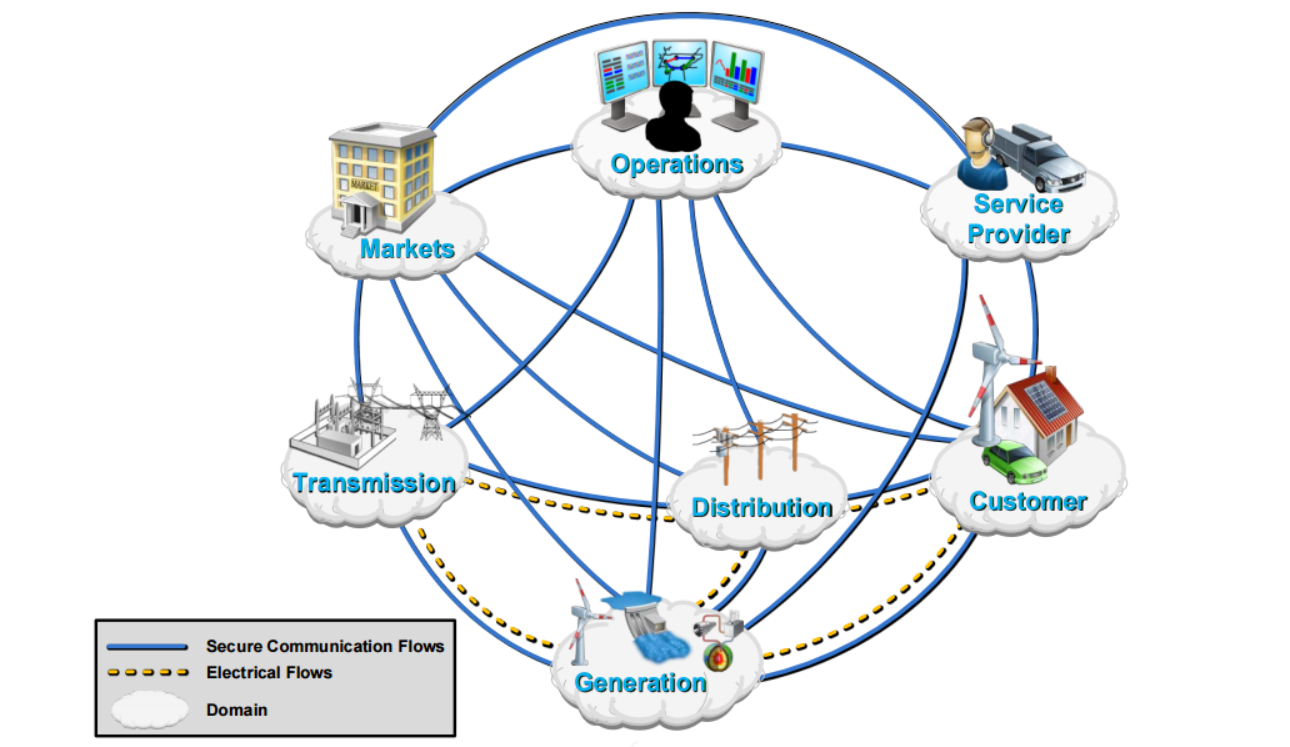
\includegraphics[width=1\textwidth]{billeder/SMARTGRID.png}
\caption{Conceptual model of smart-grid architecture. Source \fxnote{Add source}}
\label{fig:CMOSG}
\end{figure}
 
Figure \ref{fig:CMOSG} illustrates the seven domains. The seven domains each have a set of functions that is characteristic for the domain.  
 
\begin{tabularx}{\linewidth}{ r X }
Generation:& Generators of electricity. This is typically coal, oil or nuclear power plants or large-scale hydro generators. This can also include energy storage facilities that stores energy for later distribution. \\\\

Transmission:& Transmission and transformers that hold the purpose of transporting the electricity over large distances. \\\\

Distribution:& The units responsible of electricity distribution to and from the customers. \\\\

Customer:& The consumers of electricity. They may also generate electricity and sell it to the grid. \\\\

Operator:& The managers of the movement and production of electricity. They are the group that ensures that the energy is efficiently delivered where it is needed. \\\\
Market:& The sale and purchase of electricity between the different instances of the grid. One utility company could purchase power from another to keep up with demand at peek hour. \\\\
Service Provider:& The organisations providing services to the utility companies or the consumer. This could be home automation or information services.  \\
\end{tabularx}

\newpage
\section{Non-Intrusive Load Monitoring}
The operators have the responsibility of controlling the flow of energy on the smart grid. This requires the knowledge of the current consumption and a prediction about the future power requirement. This prediction is generality based on statistical data collected in the grid. If the prediction of the future power requirements can be improved, it is possible to create a better and more efficient power distribution. To accomplish this is a method known as \ab{NILM} developed.

The concept of \ab{NILM} is to use the consumption information collected at household level, and use machine learning techniques to make a qualified guess on what appliances in the household is responsible for the current consumption. By using the information from the active appliances more precise estimates of future consumption can be made. 

In today's smart grid is all customers equipped with a smart-meter. The smart-meter measures the consumption of the household, and reports it back to the smart grid. This information can be used by the markets to automatically create billing information, or by the operator to regulate the power distribution. Since this information is used for distribution regulation it is send in real-time. It is this information \ab{NILM} applications hopes to use in order to create better predictions.

\ab{NILM} can also create many opportunities for the service provider. Using \ab{NILM} it is potentially possible to gesture about the usage of each appliance in a household. This can be used to better inform the resident about power saving opportunities. Studies have shown that detailed information about energy usage, makes the resident use less energy \fxnote{ref here}. Other business opportunities, like selling the statistical information about the usage of specific appliances, also exists.  

\section{The Problem Statement}

This report seek to investigate some of the common approaches used for \ab{NILM} today, in order to determine what the capability of such approaches. It is assumed that such approaches is used in a modern smart grid setting. In order to answer this broad question, the following questions must be investigated. 

\begin{itemize}
\item	What quality of data can be expected from the smart-meters?\\
	
\item	How does errors and poor quality affect \ab{NILM} applications?\\
	
\item	What can we detect using  \ab{NILM} and where is the limits? \\
	
\item	Can anything be done to improve the \ab{NILM} technology?
\end{itemize}
If these question is answered it creates a strong foundation for gesturing about the the capability of \ab{NILM}. The main motivation for this study is not to improve grid load predictions, but to get a better basis for validate different \ab{NILM} related business opportunities for service providers. 

\subsection{The Data Approach}
To investigate the questions in the problem statement is the SmartHG dataset used. The SmartHG dataset is a collection of smart-meter data collected from 25 residential households in Denmark. The data is not filtered or cleaned en any way prior usage. This means that the data closely resembles what would be collected in a smart grid. Furthermore does the dataset contain information about the usage pattern of selected devices. This information can be used to compare inferred usage patterns to the actual. 


% 6 pages
\glsresetall 
\chapter{Data Quality}
\label{Sec:DataQuality}
Various projects today are focused on gathering data and analysing it. The gathered data is used for obtaining behaviours, habits and properties of the observed objects. This is done by using powerful statistical leaning algorithms, that are able to deduce these properties from the data. This approach is called data driven development, since the success is mainly determined by the data and not the algorithm. 

When data is the central role of the system, the quality of the data is very important. Poor data can lead to wrong assumptions, and have a negative effect on the application. Choosing the correct dataset is therefore a key factor~\cite{RefWorks:3}. Looking at the quality of the data can help chose what dataset to use. Data quality can be described many ways, one of the more formal is from the ISO 8402 standard that describes quality as: 

\begin{adjustwidth}{2.5em}{2.5em}
\emph{"The totality of characteristics of an entity that bear upon its ability of satisfy stated and implied needs"}~\cite{RefWorks:5}.
\end{adjustwidth}

This indicate that data quality is something that is very depended on the intended application, and is therefore hard to generalize. 

Quality of data is a subject that is gaining more and more attention due to the fact that the quantity of data available is larger than ever before. This forces researchers to choose between datasets. A notion of quality in the dataset can help them choose. The heavy growth in available data is a result of projects that are moving data gathering from controlled labs, to the public. Many of these projects are citizen science projects. In citizen science projects are the citizens responsible for collecting the data, and not the researchers~\cite{RefWorks:2}. This enables researchers to gather enormous amount of data, but they are no longer in control of the conditions the data are collected in. This introduces errors and other quality decreasing factors. 

\Ab{NILM} is a topic that have been in focus in the past years. This is due to the rise of the smart-meters, that makes it possible to measure at faster intervals, and collect the data on online services form real environments. But the smart-meter architecture is designed after billing and regulation purposes, and not load monitoring. The network architecture is therefore often based on the unreliable \ab{UDP}[user datagram protocol], since it is more important to get the current information fast, than get all information. This courses some of the measurements to be lost in transition, which can degrade the completeness quality of the signal. The missing data can be a problem for load monitoring, since many methods of load disaggregation are based on learning techniques. The quality of the signal can also help identify if the collected data is suitable as a training set. 


\section{Quality Criteria}
It is not uncommon that different areas of research has its own quality criteria. This is due to the fact that quality is a very domain specific subject. One of the areas that have been dealing with citizen data for many years are the Geographic information area, that are used for maps, weather prediction and climate research. They have come up with several ways of describing quality in spatial data~\cite{RefWorks:7}. Method for defining quality in time series data have also been developed~\cite{RefWorks:6}. To better define quality criteria in the smart-meter data inspiration from related work is used.

\subsection{Related Work}
Data quality is an area that recently have become a hot topic, due to the wast quantity of data. Many researchers strive to make tools that better can analyse data quality in different areas. In the area of spatial data is a \emph{"Quality and Workflow tool"} being developed by the University of Wageningen~\citep{RefWorks:8}. The objective is to help researchers select the best suited data for a given data driven project. It does this by looking at different quality criteria, given by the user or found in standards for spatial data. 

In bioinformatics is a tool named QCScreen developed to help create better dataset to metabolomics studies. In metabolomics studies are datasets often created by joining information from several different experiments of various quality. By using tools that can check the data quality and consistency to determine if a dataset is suitable for further processing, they are able to greatly improve the test results~\citep{RefWorks:9}.
 
In the article \emph{Taking a big Data approach to data quality in a citizen science project}~\citep{RefWorks:2} they talk about how quality assessment can be used to rate the believe on your data, and how to improve data collected in citizen science. The project focuses on bird observations, done by users on their smart-phones. They improve the quality by disallowing the user to send incomplete datasets to the database, and in this way forcing the user to only deliver high quality information. They then cross check the information with information from people in the same area, to see if it varies greatly. 

In the \ab{NILM} research area have data quality also emerge when talking about comparison between dataset. One of the tools working with this is the \ab{NILMTK} project~\citep{RefWorks:21}. In this they look at a series of quality parameter that can be used specifically for \ab{NILM}. They point out that looking at the energy consumption observed by the main meter in relation to what is observed at the sub-meters tells a lot about the training set. This is since the success ratio of disaggregating appliances consuming lot of energy is higher than once that only consume a little. 

One of the things all the methods have in common is trying to look at the completeness of the data. Some of the most low level criteria is the \df{sample availability}. This metric describes how many samples there is collected in relation to the expected collection amount, and look at how the samples are distributed in the measurement period. It is also seen that the \df{activity} is a good quality metric. This metric describes the amount of changes in the signal, over time. A good data set must contain both areas with high \df{activity} and areas without \df{activity}. 

\newpage

\section{Quality In SmartHG Citizen Data}
As a part of the SmartHG project 25 households have been equipped with meters on selected appliances and the main meter. The data collected from this experiment is prone with errors due to malfunctioning test equipment or unexpected interference from the resident which have resulted in offline measurement equipment for periods of time. Examples on unexpected interference could be if the resident is unplugging the measurement equipment, or turning OFF the power socket that supply's it. Unstable network does further degrade the signal, since the measurement equipment uses a lossy network. 

\subsection{Completeness And Activity}
The SmartHG data is intended for appliance recognition, and the quality must be assessed with this in mind. The completeness and the \df{activity} in the data is therefore important. 

\begin{figure}[H]
\centering
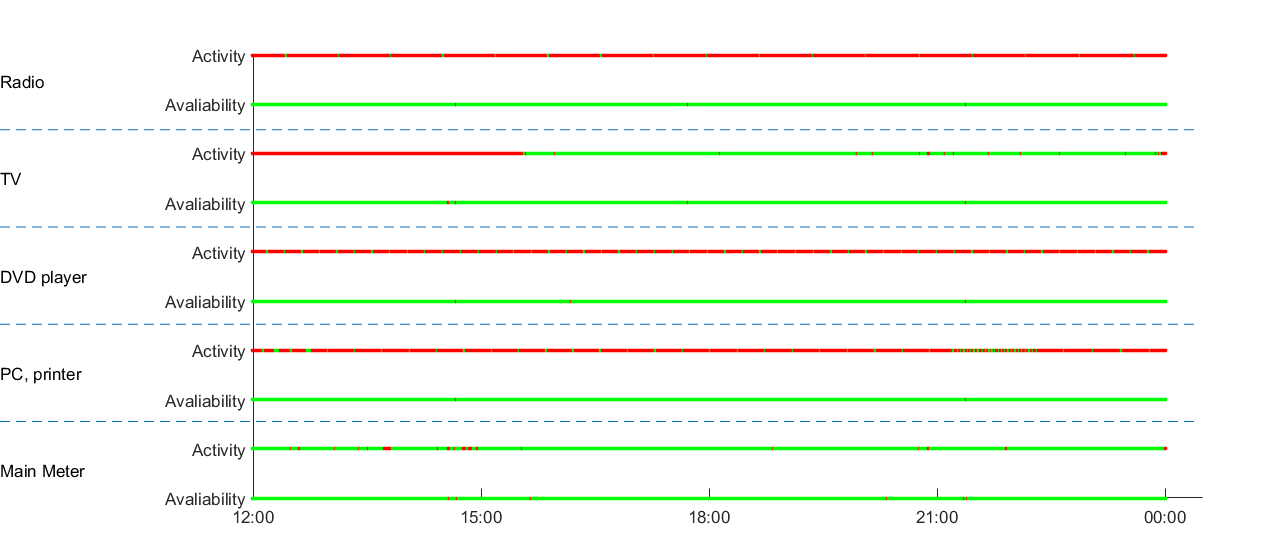
\includegraphics[width=1\textwidth]{billeder/Test.png}
\caption{12 hour overview of house 10}
\label{fig:12HRes}
\end{figure}

In Figure~\ref{fig:12HRes} is a 12 hour overview of the data in house 10 from the 16/8/2015. Here we see the \df{sample availability} and \df{activity} of the five different meters in the house. The \df{sample availability} is shown as a line where green is indicating that a sample is received as expected, and red shows a missing sample. In the figure it is shown that there is a few samples missing, which is to be expected due to the lossy network architecture. The \df{activity} is also shown as a line, where green indicates \df{activity} and red indicates no \df{activity}. \Df{activity} is measured as a change in the signal, from prior values. From this we can see that the resident have a lot of \df{activity} on the TV from around 16:00 to 00:00, which we can presume means that the television is turned ON in this period. 

First the \df{sample availability} quality of the data is assessed. The \df{sample availability} quality for a specific period of time $T_n$ for a specific meter $m$, is defined as the amount of samples observed in that timeslot over the expected sample amount. The resolution period $T_P$ for each time period in $T$ is chosen to be one hour. 

\begin{figure}[H]
\begin{picture}(0,140)
\put(0,0){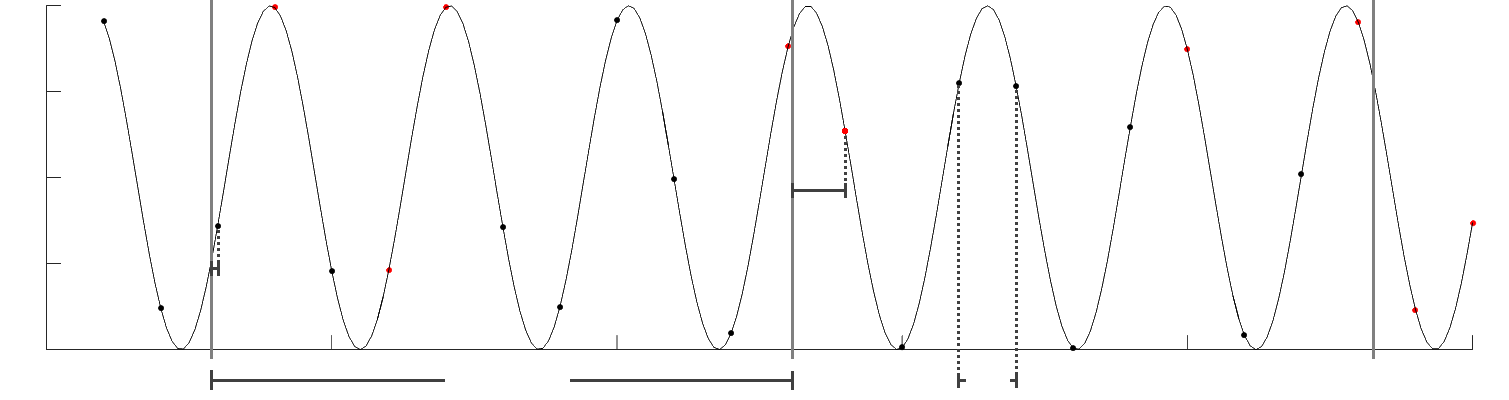
\includegraphics[width=1\textwidth]{billeder/IllustrationQua.png}}
\put(146,0){$T_P$}
\put(65,30){$\phi_{start}^{(m,T_n)}$}
\put(241,47){$\phi_{start}^{(m,T_{n+1})}$}

\put(294,0){$T_s$}

\put(145,130){$T_n$}
\put(325,130){$T_{n+1}$}

\end{picture}
\caption{Illustration of availability analysis}
\label{Fig:IOAA}
\end{figure}

To calculate the amount of samples expected to be in a specific period of time $N_{max}^{(m,T_n)}$ does the sample phase $\phi_{start}^{(m,T_n)}$ for the given period need to be known. In Figure~\ref{Fig:IOAA} is an illustration of a signal, the black dots are the samples and the red dots are the ones that are missing. The sample phase is the time from the beginning of the period $T_n$ and to the first expected sample. This is needed since for a timeslot $T_n$ of a length of $T_P$ the maximum expected sample amount can vary with 1. This is shown in Figure~\ref{Fig:IOAA} where the period $T_n$ has a potential of having 11 samples, where as period $T_{n+1}$ only can have 10. 

\begin{gather}
		N_{max}^{(m,T_n)} = \floor{ \frac{(T_{P}-\phi_{start}^{(m,T_n)})}{T_s^{(m)}}} + 1 \label{EQ:NMAX} \\
		q^{(m,T_n)} = \frac{N_{observed}^{(m,T_n)}}{ N_{max}^{(m,T_n)} } \label{EQ:QMT}
\end{gather}

As shown in Equation~\ref{EQ:NMAX} is the maximum number of samples for a meter $m$ in the period $T_n$ calculated by taking the period time $T_P$, corrected with the sample phase $\phi_{start}^{(m,T_n)}$ for the given period, and dividing it with the sample time $T_s$. The \df{sample availability} quality of the meter is calculated as the ratio of observed samples in the timeslot $T_n$ to the maximum samples, shown in Equation~\ref{EQ:QMT}. 

To find the quality of a house in a given period $T_n$, that have a set of meters $\mathbf{M}$ with a cardinality of $M$, we take the mean value of all the meter quality's, as shown in equitation~\ref{EQ:HQT}.  
\begin{equation}
	\mu_{q^{(\mathbf{M},T_n)}} = \frac{1}{M} \sum_{m \in \mathbf{M}} q^{(m,T_n)}
	\label{EQ:HQT}
\end{equation}



A quality vector $Q$ is constructed for each house. The quality vector contains the house quality found with a period $T_P$ on one hour. This have been done from March $T_1$ to October $T_N$. 

\begin{equation}
	Q^{(\mathbf{M})} = \{ \mu_{q^{(M,T)}} | T \in \{T_1, T_2, ... ,T_n,..., T_N  \} \}
	\label{EQ:HQV}
\end{equation}
This is shown in Equation~\ref{EQ:HQV} where $\mathbf{M}$ is a set of meters in a given house. This can be graphically shown in Figure~\ref{fig:SmartHGQuality} where all the houses $Q$ vectors is shown. The color is a gradient running from light green for the best quality to red for bad quality.
\begin{figure}[H]
\centering
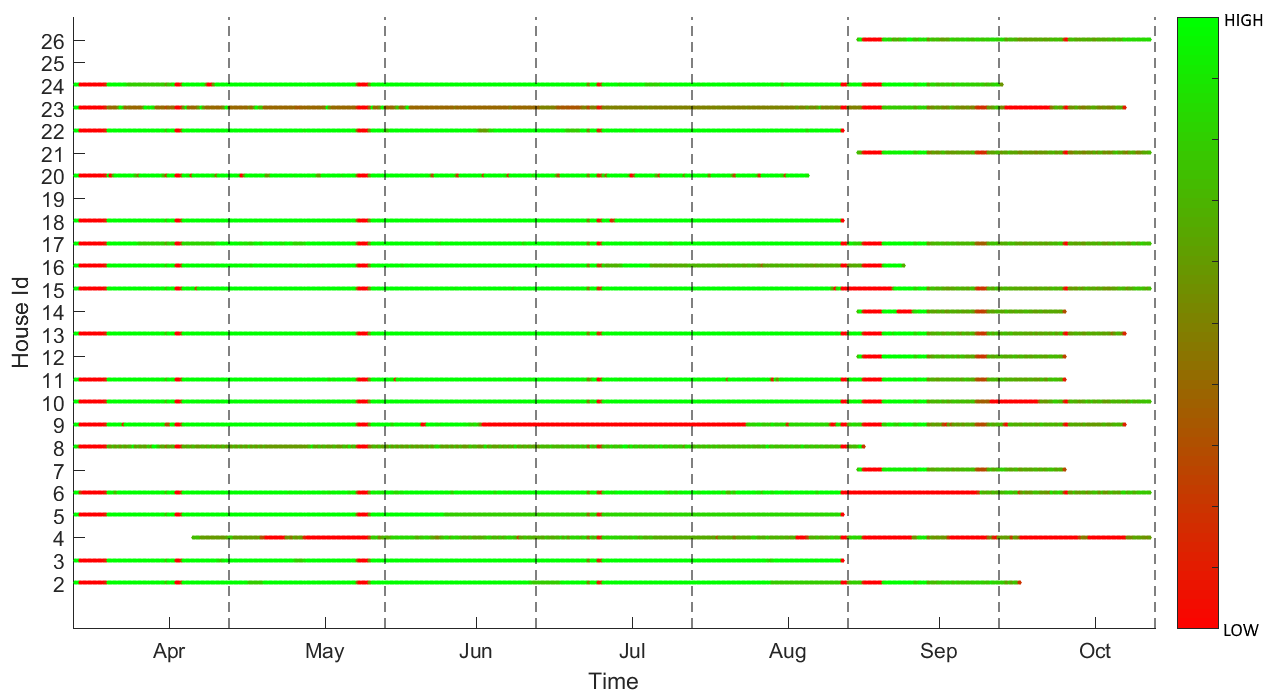
\includegraphics[width=1\textwidth]{billeder/QualityBig.png}
\caption{Quality of houses in SmartHG project}
\label{fig:SmartHGQuality}
\end{figure} 

In Figure~\ref{fig:SmartHGQuality} is the \df{sample availability} quality shown for the 25 houses in the SmartHG project. When seen on this scale with an analysis resolution on one hour it is hard to see degradation coursed by single sample missing here and there, but meters that have malfunctioned over a longer times shows itself. Since the quality of a house is the mean of several meter quality's, will this most likely appear as darker green spots, since not all meters are malfunctioning at the same time. But there still are some red areas indicating that all the meters in a house is not working. This is probably due to network problems, preventing the meters from sending the information.

There are the red spots that goes through all houses on the exact same time. This indicates that the server receiving the data for all the houses have been down, since it is unlikely that all meters in every house is down at the same time. The conclusion being that red dots most commonly are coursed by the network being unavailable so the client can not sent to the server, or the server is unable to receive. 

It is assumed that the first sample received from a meter happen at the time of meter installation, and the last sample received is the time of meter removal. The meter is assumed to be operating in between these two points in time. In the figure does the coloured $Q$ vector starts at installation time, and ends at removal time. This illustrates how some houses have been operational longer than others. A plot showing how many hours a certain percentage of meters where operating normally can be found in Appendix~\ref{APP:SampleA}. This illustrates that approximately 60\% of the time where all meters operating, without any malfunctions.

Since the data is intended for appliance recognition it is of interest where in the data there is \df{activity}, and where there is nothing happening. Both areas are impotent for a \ab{NILM} application in training scenarios. We define \df{activity} as area in the data where there is change as described in Equation~\ref{EQ:CHANGE}.

\begin{equation}
f(x) + \epsilon < f(x+1) \vee f(x) - \epsilon > f(x+1)
\label{EQ:CHANGE}
\end{equation}

Where $\epsilon$ describes a threshold to filter out changes caused by noise. This can also be described as the standard divination over an area is grater than the threshold. The \df{activity} is analysed in the available data, and is shown in Figure~\ref{fig:ActivityMap} where green is high \df{activity} and red is non \df{activity}. 

\begin{figure}[H]
\centering
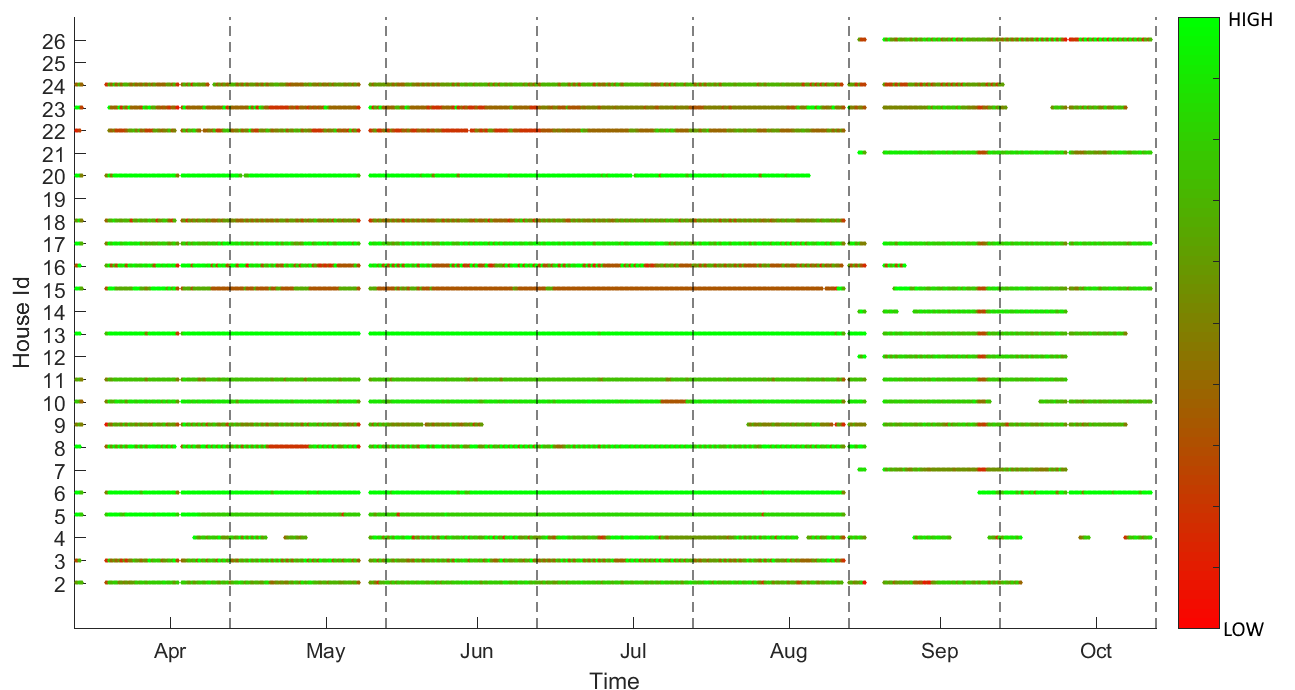
\includegraphics[width=1\textwidth]{billeder/ActivityBig.png}
\caption{Activity of houses in SmartHG project}
\label{fig:ActivityMap}
\end{figure}

The \df{activity} shown in Figure~\ref{fig:ActivityMap} is the average of the \df{activity} of the meters in the house. There is almost never a meter that does not have at least a little \df{activity} in a house, so a complete red area is fairly rare. The most interesting areas in the \df{activity} map, is often the places where there is a lot of change in the amount of \df{activity} like for house 16. The activity plot in Figure~\ref{fig:ActivityMap} and Figure~\ref{fig:SmartHGQuality} is a compact overview of the period. For a more detailed overview of the \df{activity} and \df{sample availability} see Appendix~\ref{APP:QV}. 

\subsection{Main Meter In Relation To Sub-meter Consumption}
\label{sec:MMIRTSM}
As disused in the \ab{NILMTK} project~\citep{RefWorks:21} is the relation between the energy consumption measured by the main meter and the consumption measured by the sub-meters an important quality metric. This can give two important indications about the dataset. The first indicator is how much knowledge about a house we have. A house where only a small fraction of the energy consumption is accounted for can give problems when applying \ab{NILM} algorithms. This is due to a lot of unknown consumption from other appliances. This is further discussed in Section~\ref{sec:MCACI}. The other is more appliance specific. If an appliance is not responsible for a significant part of the total consumption odds are that it is almost never ON, or that it usages so little energy that it is hard to detect. Both can have a significant impact on \ab{NILM} algorithms. This will be further discussed in Chapter~\ref{sec:AppRec} and Chapter~\ref{sec:EnvInf}.  

\begin{figure}[H]
\centering
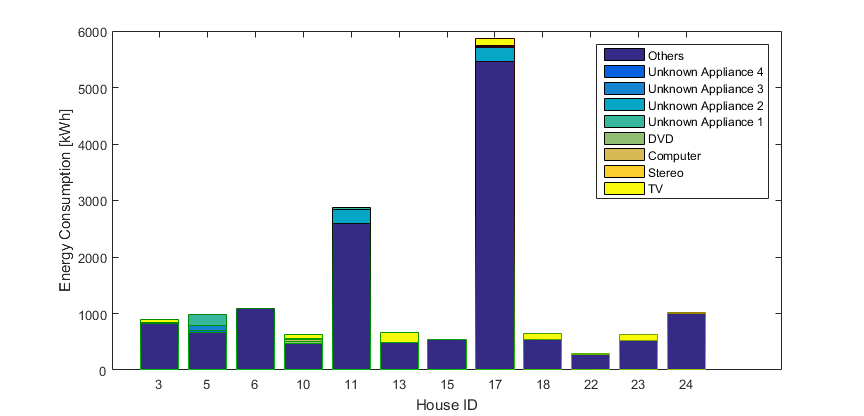
\includegraphics[width=1\textwidth]{billeder/SHGHouseUsagesV2.png}
\caption{Usage of SmartHG houses}
\label{fig:USAGEofSHG}
\end{figure}

In Figure~\ref{fig:USAGEofSHG} is the total consumption of the houses shown, and split up in the the different sub-meters, and an \df{other category}. The \df{other category} is the energy the main meter has used besides the energy accounted for by the sub-meters. In the figure is only shown the houses which main meter had observed an energy equal or greater than the sum of all the sub meters. This is not the case for houses that have malfunctioning main meters for a longer period of time, or for houses that have generated a lot of energy form solar cells. 

As seen in Figure~\ref{fig:USAGEofSHG} is the appliances equipped with sub-meters only responsible for a minor part of the total house consumption. Only the TV's and some of the unknown devices, have a relative high energy usage. The unknown devices is devices that have a sub-meter, but the appliance on the sub-meter is unknown.  

\newpage

\section{Chapter Summary}
For \ab{NILM} applications is the \df{activity} in the data, and \df{sample availability} in the data good indications of quality. Further more is the amount of energy observed by the main meter in contrast to the energy observed by the sub-meters in a house also a good indication of the dataset quality. 

In smart-grid based on a classic \ab{UDP} network architecture, can a packet loss be expected. The packet loss due to the network is shown to be relatively small. It is shown that the quality also can indicate problem in the data gathering phase of a project. problems such as malfunctioning equipment, network failure or server problems can be detected by quality monitoring systems.  

When working and gathering big amounts of data it is important to be able to gesture about the data prior to analysing it. To look at different quality measurements researchers are able to get a good general overview of the data, and find better areas to focus on. 



% 8 pages
\glsresetall
\chapter{Gap Reconstruction}
One of the more common problems in citizen science projects is gaps in data. This can happen either if the network connection is unstable or the test equipment gets prematurely turn off. This can greatly degrade the data quality, and lead to errors in the application. One way to deal with this problem is do use mathematical gap filling techniques to come with a qualified guess on how the data would look like in the gap. 

In order to use this methods we must assume that the missing data in the gap follows the same behaviour as the data on each side off the gap. Is the signal so stochastic that this is not the case gap filling is not recommended\citep{RefWorks:10}. 

In the case of the SmartHG project the data can be seen to have a part that is dependency on the previous and future data plus a stochastic part that are determined by the user and the appliance. Due to the stochastic part a perfect reconstruction is not possible, but it is the hypotheses that the non stochastic part is still so dominant that a decent reconstruction is possible. 
\section{Gaps In SmartHG Dataset}
The gaps in the SmartHG project dataset is caused by a lot of different sources. This makes the type of gaps different from case to case. Three aspects of a gap is important for the gap filling: The size of the gap, the data known before the gap, and the data known after the gap. 
\subsection{Gap Size}
Looking at the different gaps in the dataset we see that the normal gap is relatively small. This can be seen on figure \ref{fig:GapSize}
\begin{figure}[H]
\centering
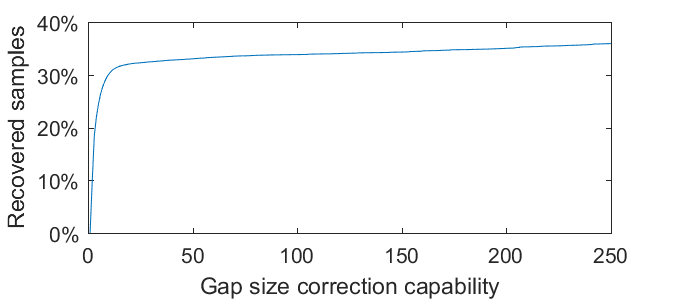
\includegraphics[width=0.8\textwidth]{billeder/CorrectionCapability.png}
\caption{Gap size}
\label{fig:GapSize}
\end{figure}
This is good since the signal part stochastic. The grater the gap, the greater influence does the stochastic part have on the signal. Smaller gaps can therefore be fixed with greater success. 
\subsection{Past And Future Availability}
It is also important how many samples are available on the left and right side of the gap. If there is a lot of gaps in the signal it can create a scenario where there only is a small amount of good data between the gaps. This makes it hard to reconstruct the data, since there is very few points to extract information about the region. 
\begin{figure}[H]
\centering
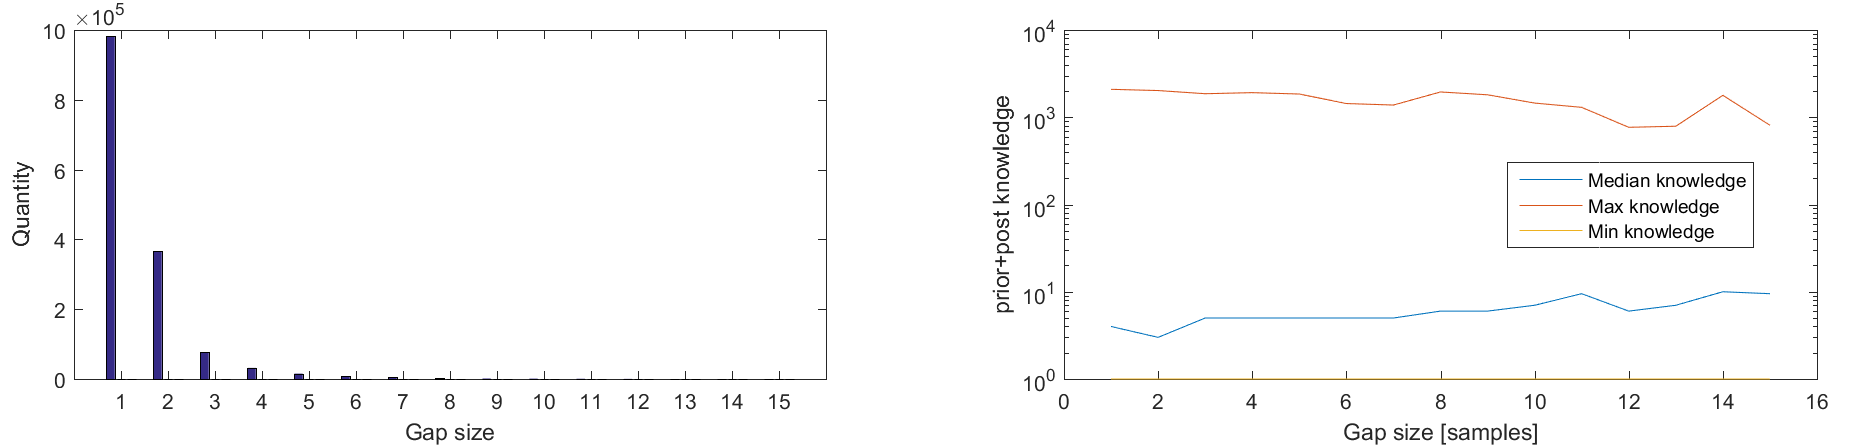
\includegraphics[width=1\textwidth]{billeder/GapInfo.png}
\caption{Past and future availability}
\label{fig:PAF}
\end{figure}
As seen on figure \ref{fig:PAF} \fxnote{Write something more when you know the result}

\section{Gap Filling Methods}
Various methods exists for gap filling. Five popular algorithms have been implemented and validated on the SmartHG project data.

\subsection{Papoulis-Gerchberg Algorithm}
\label{T:PGA}
The Papoulis-Gerchberg algorithm is a multi gap filling algorithm, meaning it is capable of correcting more than one gap at the time. This makes the algorithm preform good in conditions with many gaps and few available data points between the gaps, since it can collect information about the signal from multiple fragments signal \citep{RefWorks:11}. The Papoulis-Gerchberg algorithm works under the assumption that the signal is a periodic stationary signal whit a known bandwidth. The signal will therefore consist of $M$ frequency components, and everything outside the band is assumed to be noise. The signals in the SmartHG is not stationary, but for small snippets can approximately stationariness be assumed. 

The true bandwidth is also unknown in the signal. The Papoulis-Gerchberg algorithm is very depended on the bandwidth for a correct reconstruction. A modified version of the algorithm that estimates the bandwidth, by varying the frequency components $M$ and analysing the mean square error on the known signal is therefore used \cite{RefWorks:13}. This approach has fairly good at estimating the true value of $M$, but it is time-consuming.

\subsection{Wiener Filling Algorithm}
The Wiener filling algorithm is a extension of a Wiener predictor. Like the Wiener predictor it assumes that there exist a linear relationship between the next sample and the previous samples. By trying to predict the missing samples from both sides of the gap, and combining the knowledge it estimates the missing samples \citep{RefWorks:14}. For larger gaps does this methods rely on earlier predictions to close the gaps. This result in errors being accumulated over the gaps. The method is fast, and is therefore suited for large data with small gaps. 

\subsection{Spatio-Temporal Filling Algorithm}
The Spatio-Temporal filling algorithm uses singular spectrum analysis to split the signal into a series of sub-signals. The sum of the sub-signals are the original signal, and the sub-signals is ordered so the most dominant is first, and the least dominant is last. 

The reconstruction philosophy is that the gap has introduced noise in the signal, but a sum of only the most dominant sub-signals must be close to the original signal without noise. But in order to know how many sub-signals to include in this sum, we introduce a other artificial gap. While the sub-signals are being accumulated the mean square error of the artificial gap is observed, when this hits its peek it is assumed that the reconstruction is as good as possible \cite{RefWorks:15}.

This method is very popular for gap filling. It has shown to be very noise resistant since it finds the overall trends in the data. It does require quite a lot of data to be known post and prior to the gap, since a artificial gap must be introduced. Since it is based on singular spectrum analysis it assumes that the signal consist of stationary processes, like the Papoulis-Gerchberg Algorithm in section \ref{T:PGA}.

\subsection{Envelope Filling Algorithm}
\label{T:EGA}
Unlike the previous described methods does the Envelope filling algorithm not depend on frequency analyses, but rather on the expected power of the signal. Bye looking at the envelope of the signal it assumes that all local maxima and minima must lie on the  upper and lower envelope. It then looks at the data prior and post the gap and try to estimate the number of local maxima and minima in the gap, and their locations. It does this by looking for patterns in the time series data \citep{RefWorks:6}. When the new maxima and minima is found the points is connected by using spline \cite{RefWorks:16}. 

The methods does not make any assumptions about the signals stationariness or bandwidth. The method can also be used on none equally spaced time series. 

\subsection{Empirical Mode Decomposition Filling Algorithm}
The empirical mode decomposition filling algorithm uses empirical mode decomposition, to break the signal in to intrinsic mode functions (IMF). The sum of all IMF's is the original signal. The IMF's is all more low frequent ans simpler in structure than the original signal. The hypothesis is that it is easier fixing a gap in a simple signal than a complex one. 

The envelope filling algorithm in section \ref{T:EGA} is used to fix the gaps in the IMF's. The IMF's can now be accumulated to get the original fixed signal. Like the envelope filling algorithm does it not make any assumptions about the signals stationariness, bandwidth and can be used on none equally spaced time series. But making a empirical mode decomposition on a signal with a gap in is a non trivial process and can introduce errors \citep{RefWorks:16}. 

\section{SmartHG Dataset Reconstruction}

\section{Related Work} 

% 19 pages
\glsresetall
\chapter{Appliance Recognition }

Appliance recognition and load disaggregation is some of the key aspects in non intrusive load monitoring (NILM). The main purpose of the NILM approach is to better understand the power usage in home, and help the different household to more optimal power savings. This is done by informing the residents about the power consumption of individual appliances. It is shown that informing a household about its usages pattern can lead to savings \fxnote{find a ref for this}. This makes the basis for load disaggregation, where appliance specific load is guessed based on the main meter load. This enables the user to know what uses the energy and when.

One other aspect of NILM is event detection. Sometime the actual consumption of an appliance is not as important as when it was used, and for how long. This is a simpler task than guessing the true consumption, and is for some applications a better approach. As an example is this kind of information sufficient if we want to track the activity of a elderly person in a assisted living situation \fxnote{find a ref for this}. 

\section{NILM Concepts And Challenges} 
The aim of NILM is to partition the hole house consumption data in to appliance specific consumption. 
\begin{equation}
	P(t) = p_1(t) + p_2(t) + ... + p_n(t)
	\label{EQ:PAC}
\end{equation}
This can be seen as in equation \ref{EQ:PAC} where $P(t)$ is the total consumption at time $t$, and $p_n(t)$ is the consumption of appliance $n$ at time $t$. The aim is to partition $P(t)$ back to the different appliance specific consumptions. In order to structure the problem we categorise the appliances in 3 groups \fxnote{ref her til a}: 

\begin{tabularx}{\linewidth}{ r X }
Type-I:&Appliances that only have 2 states corresponding to on/off. This could be a lamp or a water boiler. \\
\\
Type-II:&These are appliances with multiple states, and can be modelled as a finite state machine. Many modern devices such as TV's, computers and washing machines fall in this category.   \\
\end{tabularx}

\begin{tabularx}{\linewidth}{ r X }
Type-III:&These are appliances is referred to as Continuously Variable
Devices. These devices have a variable power draw and is impossible to model as a finite state machine. This could be appliances like power drills, and dimmer lights. These are by far the hardest for the NILM algorithms to detect. \\
\\
Type-IV:& These are a special kind of appliances that are always on and consume energy at a constant rate. Such devices could be smoke detectors and TV receivers.  \\
\end{tabularx}

Some of the different appliance types is illustrated on figure \ref{fig:ATO}. 


\begin{figure}[H]
\centering
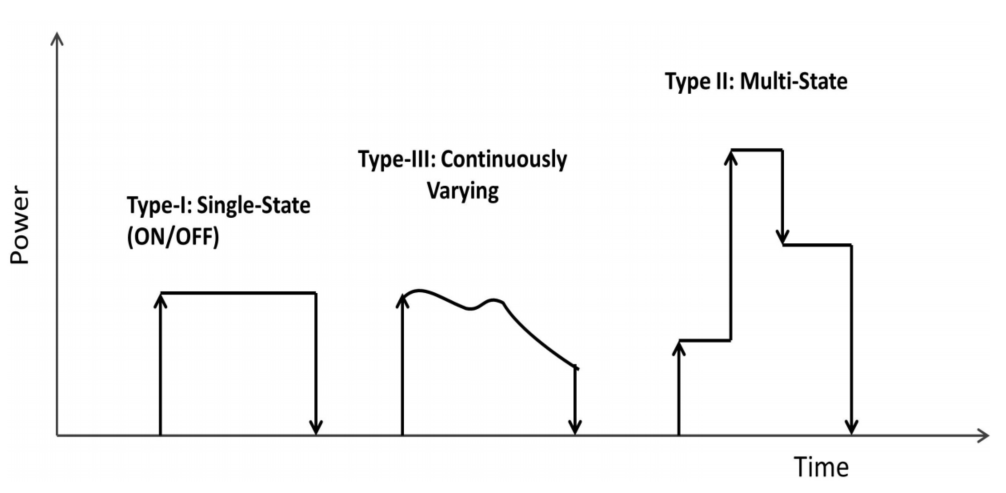
\includegraphics[width=0.6\textwidth]{billeder/Types.png}
\caption{Appliance types. Source \citep{RefWorks:17}}
\label{fig:ATO}
\end{figure}

The appliances in Type-IV is not a particular researched area, since it does not give the user much information to calculate savings from. These appliances is often using very little energy, and must not be turn off at will. 

Type-I and Type-II are very used, and can cover all most any appliance. In the area of event detection are the most common approach to see all appliances as Type-I appliances and detecting on/off events. Most appliances today is Type-II appliances due to growing amount of complicated electronics that are embedded in them. Then there are devices that are Type-II but most of the time act like Type-I appliances. An example of this is the vacuum cleaner. On most vacuum cleaners you are able to change the suction intensity, which makes it type two. But most people don't change this very often, so the energy usage looks more like a Type-I appliance. 
 
\subsection{NILM Features} 
For data disaggregation it is common to use method based in machine learning and optimization. The approach is to first extract features from the dataset, and then train or validate by using this features. 

In NILM the features can be sub categorised in steady state, transient state and non-Traditional features.  These categories can be further expanded as shown on figure \ref{fig:FTR}. 

\begin{figure}[H]
\centering
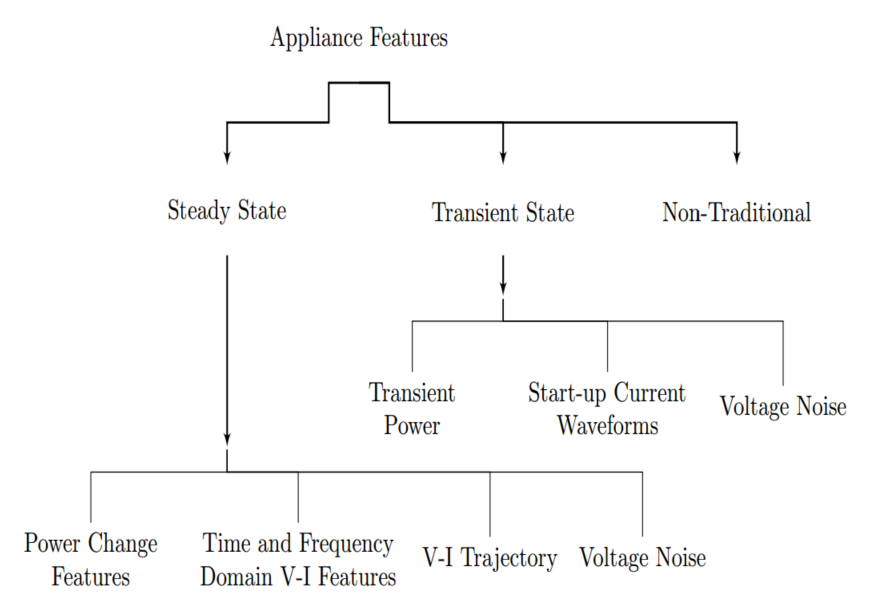
\includegraphics[width=0.6\textwidth]{billeder/featureOverview.png}
\caption{Feature types. Source \citep{RefWorks:17}}
\label{fig:FTR}
\end{figure}

Steady state features is features that can be extracted when the signal is in the stable state. Features that are often extracted in this state is "Power Change" which is the jump in power or reactive power usage. Time and frequency analysis is often used on the voltage and power signals of the meters. It is shown that analysing the harmonics in signals is a powerful way of making appliance detection \citep{RefWorks:29}.The trajectory between voltage and power usage is a god feature. This can be used to detect the reactive power of a signal, which is a give-away for inductive loads. Some researchers have shown that different appliances makes different noise profiles on the main line. Unfortunately does this kind of recognition require a extremely high sampling rate \citep{RefWorks:30}. 

The transient state of an appliance is a short state that comes when a appliance switches between steady states. In this state there often is appliance semi-unique waveforms in the current and voltage domain. The noise generated on the mainline in this state is also a good indication of the appliances type. 

There also exists a series of non-traditional features, that is used in special types of algorithms. One of them is based on matching the power usage profile to geometrical figures, and using the series of figures to recognize an appliance \citep{RefWorks:17}.  

Many of the above features requires a high sample rate in kHz or Mhz span in order to be effective. This is often not the case, since it is normal smart meters that are providing the data. For a smart meter a sample rate at 1 Hz would be considered fast, and for many applications this is down to $0.03$ Hz or slower. It is therefore common only to use the steady state features, and most of the time only the power change feature, which looks at changes in power, reactive power, current or voltage. 

\subsection{Learning Strategy} 
When you have extracted features from the signal there are several algorithms there can be selected for the training. They can roughly be split up in two categories optimization algorithms and machine learning algorithms. The optimization algorithms relies on a database of appliance info, and tries to find the subset of the database that are most likely to be in use. 

\begin{equation}
	M = \argmin_{x \in \powerset{D} } \left( \mid {\sum_{i = 0}^{I} x_i - \hat{y}  \mid} \right)
	\label{EQ:OMP}
\end{equation}

This is illustrated in equation \ref{EQ:OMP} were a set of appliances $M$ that correspond to the measured signal $\hat{y}$ needed to be found. This is achieved by searching the known database of all appliances $D$. This is done by taking the powerset of the database and finding the subset that minimises the error. This approach is fine for a small amounts of appliances, but for large databases and many appliances in use at the same time, does this take far to long to be practical. 

Due to this, most researchers use pattern recognition techniques instead. These have the benefits of being more scalable, and be usable even if only parts of the device database is known. There are generality two approaches to pattern recognition: supervised and non-supervised. In supervised training it is assumed that the ground truth of your system is known. For a NILM application this means that the true consumption of the appliance need to be available for the training process. This means that a sub meter must be placed to measure the appliances individually, which often is costly and time consuming. In non-supervised methods, is only the main meter readings available, and no information about the appliances are known. This type of algorithms will usually try to cluster the readings in distinct groups cosponsoring to a guess of what appliances that correspond to the reading. Fore this kind of training it is easy to collect a big training set, but it requires the groups to be manually labelled afterwards.  
  
Most algorithms are based on clustering techniques and hidden Markov models. Hidden Markov models have proven very effective when classifying Type-I and Type-II appliances. This is due to its ability to model state changes as a imported part of the classification. It is shown that using clustering techniques can greatly improve the classification, and reduce the training time. Artificial neural networks is also showing great promise, and is a topic that is currently in focus by many NILM researchers. More on this in section \ref{sec:RecRelatedwork}. 

\subsection{NILM Challenges} 
There are many challenges in NILM. One is the Type-III appliances. Due to there varying, and at time random, energy consumption it is hard to fit them to a behavioural model. This is made further harder by the low sample rate. Many great features of the appliances is hidden due to the low sample rate most data is collected with\citep{RefWorks:17}.

A other problem is the "heavy consumer problem". In a house there are some appliances that require a lot of energy when they are on, such as stoves, air conditioners and refrigerators. These is often refereed to as the heavy consumers. Then there is the appliances that consumes very little energy like laptops, DVD players and routers. The heavy consumer problem is that the heavy consumers is so dominant that they make it hard to track the power signature of little consumers. This is why many researchers only focus on the top 10 heavy consumers when during NILM applications \citep{RefWorks:21}. 

\section{Related Work} 
\label{sec:RecRelatedwork}

There are several interesting problems and approaches being researched in the NILM community in the moment. One is the lag of a good bases of comparison, both to compare the performance and the training time of a solution. It was a common practise that each researcher uses his own dataset, or an artificial lab setting to validate the results. This made it hard to compare the algorithm to others, and raised questions about the correctness of the findings. \\
To accommodate this problem the NILM-Toolkit was created. This is a collection of python library's, that create a framework to evaluate NILM solutions. It supports a wide range of known datasets that can be used to train or validate an algorithm. It also comes with two benchmark algorithms to be used to compare a new algorithm against. The NILM-Toolkit will help researchers to easer share and compare algorithms in the future\citep{RefWorks:21}. 

Another framework to accomplish better comparison and sharing is the NILM-eval framework. This is based on Matlab and supports algorithms to be written in either Matlab or in python. The NILM-eval and the NILM-Toolkit is created to solve the same problem, and is compatible with each other in the sense that the interface for algorithms are the same\citep{RefWorks:26}. 

Deep neural networks have last yeas improved the are of computer vision and speech recognition remarkably. NILM researchers are starting to look in to if similar techniques can be used to improve data disaggregation. Neural nets have like hidden Markov models the ability to model state changes. Furthermore they are capable of automatically finding important features in the data. Preliminary tests shows that a deep neural net can out preform the classic hidden Markov model approaches. The downside with the deep neural network is that it takes weeks to train, and there are thousands of parameters there can be changed. This makes the task of finding the global minimum hard, and the method is very prone to be stuck in a local minimum. The method is currently being used on heavy consumers\citep{RefWorks:25}. Current research is looking that its potential in solving the heavy consumer problem, but no definite conclusions is yet to be reached. 

Many approaches is supervised, since this kind of approach is better at separating the appliances. But this require that you first build a database with information about all the appliances. To have this prior knowledge of the system seems unrealistic in a application setting, where it is most likely you do not know anything about the house. To combat this various unsupervised methods have been developed. The focus in this kind of studies have been load separation for the sake of making power savings, or to inform the electric companies to help them create a more stable electric grid. There are several good algorithms for this today that support this purpose. For event detection and user habits analysis it is still most common to use the supervised approaches \citep{RefWorks:19}. This paper will therefore focus on the supervised approaches. 

\newpage
			

\section{Recognition Methods} 
Methods based on Hidden Markov models is currently the most popular method for NILM. Three method is selected to be validated in this paper. The methods are selected since they are often refereed to in literature, and is often used as benchmark algorithms. All of the algorithms is based on hidden Markov models in different configurations. In the following subsections will the algorithm be briefly explained. 

\subsection{Factorial Hidden Markov Models}
The hidden Markov models has proven to be one of the most used tools to create probabilistic models based on time series data. This is done by seeing the system as a series of observable states $Y_t$, and a series of hidden states $S_t$ \citep{RefWorks:20}. It is assumed that there excites a probabilistic relation between the observations $Y_t$ and a sequence of hidden states $S_t$. This is implemented as a first order model, which implies that the current hidden state $S_t$ is only depended on the previously state $S_{t-1}$ and the current observed state $Y_t$. It is the dependency to previously states that makes it grate for time series.  

\begin{equation}
	P(\{ S_t, Y_t \} ) = P(S_1)P(Y_1 | S_1) \prod_{t=2}^T P(S_t|S_{t-1})P(Y_t|S_t)
	\label{EQ:HMM}
\end{equation}

The joint probability for a specific hidden state $S_t$ have caused the output $Y_t$ can be seen in equation \ref{EQ:HMM}. $P(Y_t|S_t)$ is the observation probability, which shows that conditional probability for $Y_t$ is outputted given the hidden state $S_t$. The probability for a state change is given by the transition property $P(S_t|S_{t-1})$. 

Factorial hidden Markov models is an extension of this classic hidden Markov model where there exists several hidden state chains that all contribute to the observed output. This can be seen as an extension to equation \ref{EQ:HMM} where the hidden states $S_t$ can be seen as a series of states as shown on equation \ref{EQ:FHMM} where $M$ is the number of chains.

\begin{equation}
	S_t = \{ S_t^{(1)}, ..., S_t^{(m)}, ...., S_t^{(M)} \}
	\label{EQ:FHMM}
\end{equation}

This can also be shown graphically on figure \ref{fig:FHMM}. Here we see how three chains all contribute to one output. 

\begin{figure}[H]
\centering
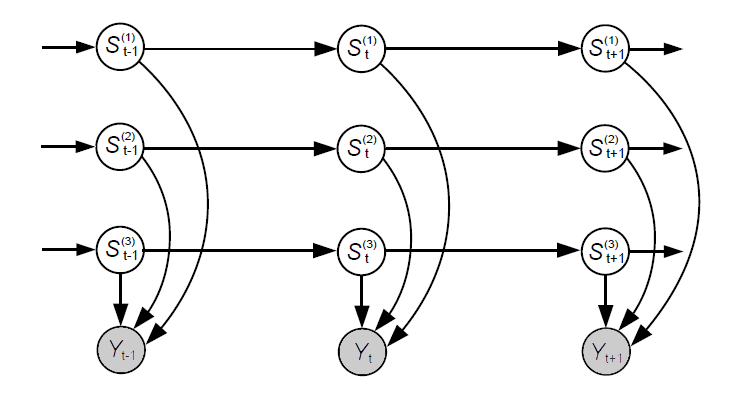
\includegraphics[width=0.8\textwidth]{billeder/FHMM.png}
\caption{Factorial hidden Markov model illustration. Source \citep{RefWorks:20}}
\label{fig:FHMM}
\end{figure}

As a extra constrain must each hidden state in in each chain only is depended on the previously state in the chain, and do not depend on the hidden state of other chains. This makes the state transition probability to be defined as in equation \ref{EQ:CTP}. 

\begin{equation}
	P(S_t|S_{t-1}) = \prod_{m = 1}^M P\left( S_t^{(m)}| S_{t-1}^{(m)} \right)
	\label{EQ:CTP}
\end{equation}

The observed stated can therefore be seen as the sum of fractions of the different chains. 

In this implementation there is normally used only two or three states, since most appliances is seen as Type-I or Type-II appliances. There is trained one chain for each of the appliances plus one that is called the other chain. This chain is to allow for the other appliances that are not taken in to the model and noise. The model can therefore be used to validate for a given output what is the probability that a given appliance is contributing to the output. The concrete implementation for this algorithm has been borrowed from the NILM-Toolkit \citep{RefWorks:21}. 

\subsection{Parson}
The Parson algorithem is a variant of the Kolter and Jaakkola algorithem\citep{RefWorks:22}. The algorithm is designed to be a semi-supervised learning algorithms. This means that the algorithm does not need to train on the data from the concrete house prior to deployment, but it still requires some prior knowledge. The idea is to have a database of general appliance models, that tells how specific appliances most likely will behave. This model will be able to detect the device, and do some unsupervised special training to better fit the concrete appliance. 

The algorithm is based on a kind of HMM called "difference HMM" since they take the step difference in the aggregated data and use as the observed output $Y_t$. In a normal hidden Markov model there is only emitted one output for each hidden state in a chain. In the Parson algorithm the model is changed to output two states from the hidden states $X_t$ and $Y$. This creates a model structure that can be graphically illustrated as on figure \ref{Fig:ParsonModel}\citep{RefWorks:28}. 

\begin{figure}[H]
\begin{picture}(0,140)
\put(90,0){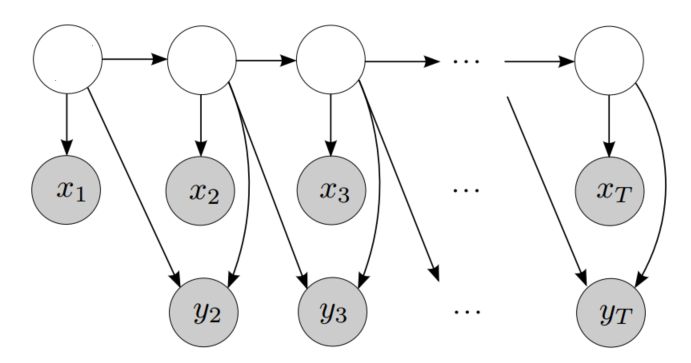
\includegraphics[width=0.6\textwidth]{billeder/ParsonIlu.png}}
\put(112,115){$S_1$}
\put(165,115){$S_2$}
\put(215,115){$S_3$}
\put(326,115){$S_T$}
\end{picture}
\caption{Parson hidden Markov model structure. Source \citep{RefWorks:28}}
\label{Fig:ParsonModel}
\end{figure}

The $Y_t$ is corresponding to the step in power that is observed since the last sample. It is assumed that the only thing that can cause a step in power if is an appliance changes states from one to another. The $X_t$ is the mean constant power draw of the state. This is used to filter out the appliance if the power draw observed is smaller than this threshold.

It is assumed that the power consumption of a state in the general model of an appliance can be modelled as a Gaussian. This can be illustrated as in equation \ref{EQ:GPF}. 

\begin{equation}
	P(X_t|S_t) \rightarrow \mathcal{N}( \mu_{S_t} , \sigma_{S_t}^2 )
	\label{EQ:GPF}
\end{equation}

This shows how the power draw of a appliance is modelled as Gaussians. The step change emission probability $Y_t$, can be seen as a Gaussian that is created from the change between two states as shown in equation \ref{EQ:GST}.

\begin{equation}
	P(Y_t|S_t, S_{t-1}) \rightarrow \mathcal{N}( \mu_{S_t} - \mu_{S_{t-1}} , \sigma_{S_t}^2 + \sigma_{S_{t-1}}^2 )
	\label{EQ:GST}
\end{equation}

To model the constraint that the meter only can be on if the mean power draw is present in the signal is a additional constraint added to the emission probability. This constrain is mathematically described in equation \ref{EQ:PCA}.

\begin{equation}
	P(w_{S_t} \leq x_t | S_t ) = \int_{-\infty}^{x_t}  \mathcal{N}( \mu_{S_t} , \sigma_{S_t}^2 ) dw
	\label{EQ:PCA}
\end{equation}

Where $x_t$ is the measured power consumption and $w_{S_t}$ is the appliance power draw constraint. This makes the probobility going towards zero if the total power draw is to little and towards 1 if there is more than enough power. This is a loose constraint since too high power draw also could be created by other appliances. To minimise the impact this have for the algorithm is the mean power draw subtracted from the data before other appliances is searched for. 

In the implementation validated in this paper all appliances is modelled as Type-I. The algorithm is allowed to train on the house data, to better fit the general models to the appliances. 

\subsection{Weiss}
The algorithm proposed by Weiss called "AppliSense" is a other approach that do not use Markov models\citep{RefWorks:23}. The philosophy is that some appliances like lamps and kettles are purely resistive, where others like washing machines and air conditions is more inductive and some appliances like laptops is more capacitive. Bye measuring not only the power consumption, but also the amount of reactive power it is revealed if there is inductive or capacitive appliances.

The algorithm is supervised since it requires a signature database to be created prior to usage. The signature database consists of how the changes will be in reactive and real power for a specific device when it is turned on and off. In their paper the authors show a method where this database can be created of a user, by using a smart-phone application and turning on and off appliances in the house, and inputting the information in the mobile application\citep{RefWorks:23}. In this paper the database is created by data collected from the sub-meters measuring only the devices.  

The algorithm looks for significant power changes in the data. If a change is found it is assumed to be an on or off event. The change is now compared to all the values in the database. If a close match is found it is assumed to be this device, if not it is a unknown device. This limits the approach to Type-I appliances, and the algorithm requires the reactive power to be measured. 

\section{The ECO Dataset}
The experiments in this section will be done on the "Electricity Consumption and Occupancy" (ECO) dataset \citep{RefWorks:26}\citep{RefWorks:27}. The dataset consists of six houses that have been equipped with sub-meters on selected meters and the main meter. The data is collected in Switzerland in the period June 2012 to January 2012. 

The data is sampled with a resolution on 1 Hz on both the sub-meters and the main meter. On the main meter is both real and reactive power measured, where on the sub-meter it is only the real power. 

\begin{figure}[H]
\centering
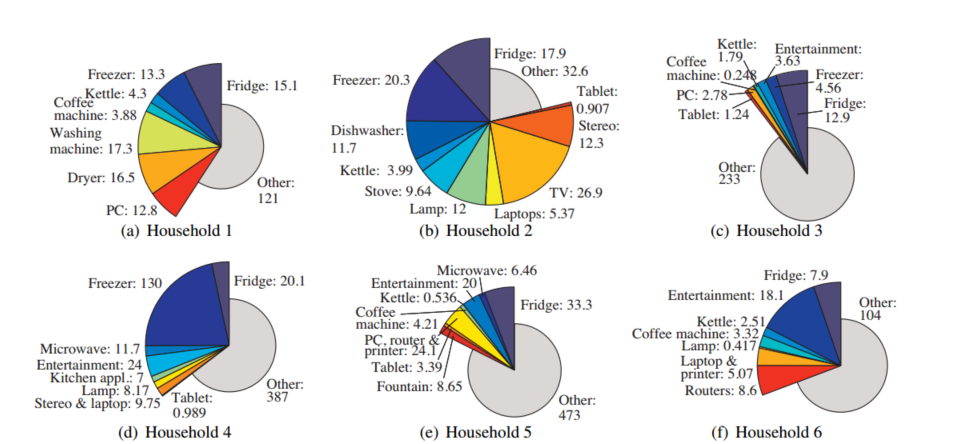
\includegraphics[width=1\textwidth]{billeder/ECOHouses.png}
\caption{House energy distribution. Source \citep{RefWorks:26}}
\label{fig:EHD}
\end{figure}

On figure \ref{fig:EHD} is shown how different appliances are responsible for the energy consumption in the different houses, in the ECO dataset. Here we see that for house two is more than $75\%$ of the energy usages accounted for by the sub-meters. This makes house two a preferred candidate for experiments, since we know who is the the heavy consumers and who is the little consumers.  

\section{Validation of Methods} 
\lipsum[3]
% Validate 

\subsection{Sample rate experiment}
% Gradiunality 
\lipsum[4]
\subsection{Gap filling experiment}
% Gap 
\lipsum[5] 

% 14 pages
\glsresetall
\chapter{Environment Influence } 
\label{sec:EnvInf}
Not just the sample rate and error ratio are determining factors when designing a \ab{NILM} application. The environment which the application is deployed and trained in is critical for the performance of the system. 

The environment is the parameters describing the static conditions of the household which the algorithms are deployed in. An example of an environment parameter can be number of known devices, number of unknown devices, number of simultaneously active devices or number of training days. In order to investigate some of the environment parameters effect on a \ab{NILM} application the SmartHG dataset is used. 

\section{Challenges In The SmartHG Dataset} 
The \ab{ECO} dataset, consists of 6 households and the data is sampled at a rate of 1 Hz over a period of 8 months. The SmartHG dataset is different in many aspects. The data is sampled at a slower rate of $\frac{1}{30}$ Hz, but on 25 households over a period of 6 month. Each house have only a small number of sub-meters. The sub-meters are mainly placed on little consumers such as televisions and stereos, which presents an interesting challenge for load disaggregation. The SmartHG dataset contains both the aggregated data, and the instantaneous power usages of the different households.

\begin{figure}[H]
\centering
\includegraphics[width=1\textwidth]{billeder/TotalPie.png}
\caption{Frequency comparison of the reconstruction methods}
\label{fig:SLC}
\end{figure}

In figure \ref{fig:SLC} is the power distribution of three households shown. This illustrates how much energy each appliance uses, in relation to the households total energy consumption. The "other" category shows the energy consumption not accounted for by the sub-meters.  

Household 3,10 and 18 are some of the houses that have the smallest "other" category. They are therefore selected for further study, since they provide the most information about the house. 

\section{Appliance Noise Influence On Detection }
\label{sec:AppNoise}
The households in the SmartHG dataset have a relative big consumption created by other appliances than the ones with a sub-meter. This consumption can be thought of as "appliance noise", since it is a signal that is not included in the disaggregation model. 

\subsection{Detection In A Noisy Environment }
\label{sec:NOISE}
To investigate the influence appliance noise have on a \ab{NILM} application, disaggregation of the known appliances of house 3, 10 and 18 are done using the Parson and \ab{FHMM} algorithm. 

\begin{table}[H]                             
\centering                                   
\begin{tabular}{cc|c|c|c|c|}
\cline{3-6}
\multicolumn{1}{l}{}                            &        & \multicolumn{2}{c|}{FHMM} & \multicolumn{2}{c|}{Parson} \\ \cline{3-6} 
\multicolumn{1}{l}{}                            &        & F1        & Accuracy      & F1         & Accuracy       \\ \hline
\multicolumn{1}{|c|}{\multirow{3}{*}{House 3}}  & TV 1   & 0.19      & 0.74          & 0.10       & 0.40           \\ \cline{2-6} 
\multicolumn{1}{|c|}{}                          & PC     & 0.19      & 0.84          & 0.13       & 0.45           \\ \cline{2-6} 
\multicolumn{1}{|c|}{}                          & TV 2   & 0.03      & 0.84          & 0.20       & 0.11           \\ \hline
\multicolumn{1}{|c|}{\multirow{4}{*}{House 10}} & TV 1   & 0.60      & 0.76          & 0.40       & 0.25           \\ \cline{2-6} 
\multicolumn{1}{|c|}{}                          & Stereo & -         & 1.00          & -          & 1.00           \\ \cline{2-6} 
\multicolumn{1}{|c|}{}                          & PC     & -         & 0.99          & -          & 0.99           \\ \cline{2-6} 
\multicolumn{1}{|c|}{}                          & TV 2   & -         & 0.99          & -          & 0.99           \\ \hline
\multicolumn{1}{|c|}{\multirow{3}{*}{House 18}} & TV 1   & 0.36      & 0.65          & 0.24       & 0.14           \\ \cline{2-6} 
\multicolumn{1}{|c|}{}                          & Lamp   & -         & 0.99          & -          & -              \\ \cline{2-6} 
\multicolumn{1}{|c|}{}                          & TV 2   & 0.73      & 0.58          & -          & 0.00           \\ \hline
\end{tabular}                               
\caption{Appliance disaggregation results of house 3,10 and 18 for the SmartHG dataset.}                     
\label{table:Tab:SHGREAL}                    
\end{table}                   

On table \ref{table:Tab:SHGREAL} is the results from the disaggregation shown. The low F1 scores indicates that it is hard for the algorithms to correctly disaggregate the meters. This is due to the many spikes there are in the data that can indicate a change in appliance usage. On figure \ref{fig:RMD} is a snippet from the validation period shown. The blue line shows the data from the main meter. The other lines indicates the appliances. On the left side of the figure is the true consumption shown for all the meters. This consumption is known from the sub-meters on the appliances. On the right side is the true main meter signal shown, and the inferred usages of the different appliances created by the \ab{FHMM} algorithm. 

\begin{figure}[H]
\begin{picture}(0,150)
\put(0,10){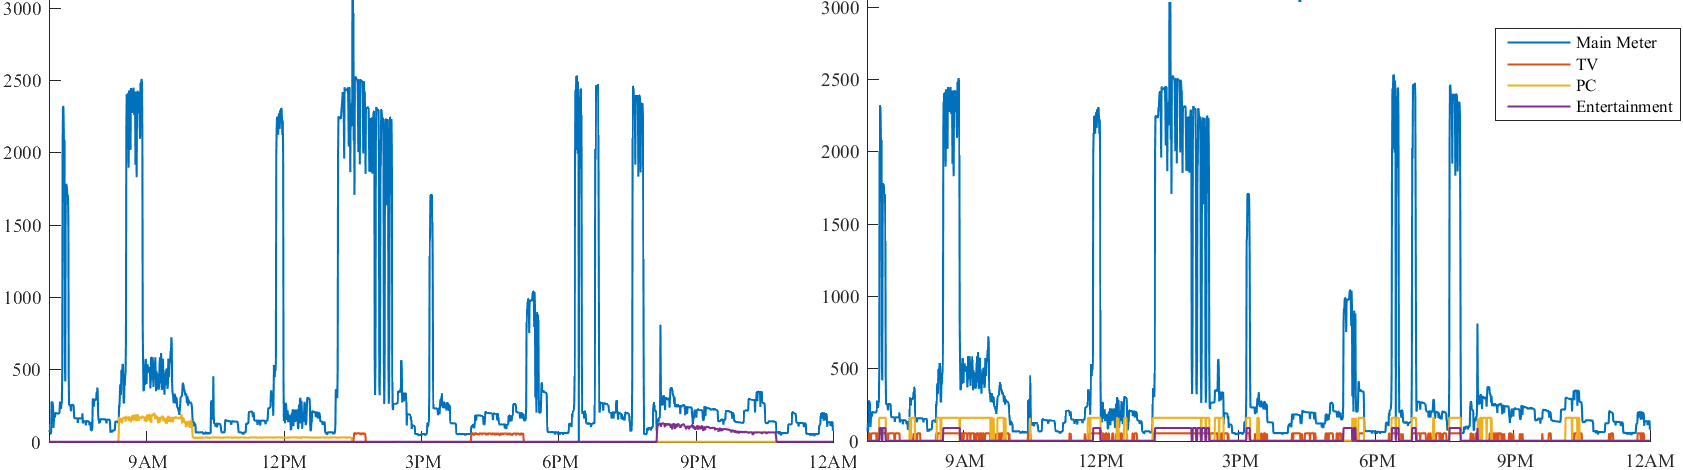
\includegraphics[width=1\textwidth]{billeder/RecognitionEx1.png}}

\put(90,140){True Signals}
\put(300,140){Inferred Signal}

\put(-10,65){\rotatebox{90}{Watt}}
\put(215,0){Time}

\end{picture}
\caption{FHMM disaggregation snippet}
\label{fig:RMD}
\end{figure}

On the figure is shown how the main meter have many fluctuations. The algorithm tries to map each fluctuation to a change in an appliance, or noise. There are many of the noise fluctuations that are similar to the appliance changes, and this creates errors in the disaggregation. 

\subsection{Detection In Noise Free Environment }
\label{sec:NOISEFREE}
The assumption that the noise is what troubles the disaggregation, dictates that for a house where all appliances are known, and therefore there are no noise, will preform better. 

\begin{figure}[H]
\centering
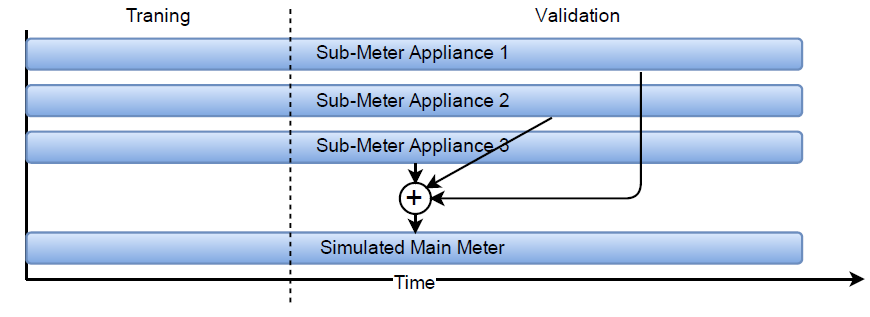
\includegraphics[width=1\textwidth]{billeder/SimIllu.png}
\caption{Artificially constructed main meter}
\label{fig:SIL}
\end{figure}

In order to test this hypothesis is a main meter signal artificially constructed by summing the values of all the sub-meters in a house as illustrated on figure \ref{fig:SIL}. In this manner is a new set of artificial houses created where there are no appliance noise. By applying the same disaggregation algorithms, as for the noisy environment, on the noise free environment is the performance much increased as shown in table \ref{table:Tab:SHGSIM}.

\begin{table}[H]                             
\centering                                   
\begin{tabular}{cc|c|c|c|c|}
\cline{3-6}
                                                &        & \multicolumn{2}{c|}{FHMM} & \multicolumn{2}{c|}{Parson} \\ \cline{3-6} 
                                                &        & F1        & Accuracy      & F1         & Accuracy       \\ \hline
\multicolumn{1}{|c|}{\multirow{3}{*}{House 3}}  & TV 1   & 0.73      & 0.96          & 0.26       & 0.86           \\ \cline{2-6} 
\multicolumn{1}{|c|}{}                          & PC     & 0.74      & 0.96          & 0.30       & 0.91           \\ \cline{2-6} 
\multicolumn{1}{|c|}{}                          & TV 2   & 0.83      & 0.96          & 0.20       & 0.11           \\ \hline
\multicolumn{1}{|c|}{\multirow{4}{*}{House 10}} & TV 1   & 0.97      & 0.98          & 0.40       & 0.25           \\ \cline{2-6} 
\multicolumn{1}{|c|}{}                          & Stereo & -         & 1.00          & -          & 1.00           \\ \cline{2-6} 
\multicolumn{1}{|c|}{}                          & PC     & -         & 0.99          & -          & 0.99           \\ \cline{2-6} 
\multicolumn{1}{|c|}{}                          & TV 2   & -         & 0.99          & -          & 0.99           \\ \hline
\multicolumn{1}{|c|}{\multirow{3}{*}{House 18}} & TV 1   & 0.95      & 0.98          & 0.24       & 0.14           \\ \cline{2-6} 
\multicolumn{1}{|c|}{}                          & Lamp   & -         & 0.99          & -          & -              \\ \cline{2-6} 
\multicolumn{1}{|c|}{}                          & TV 2   & 0.73      & 0.58          & 0.73       & 0.58           \\ \hline
\end{tabular}                              
\caption{Disaggregation of appliances on artificially constructed main meters }                     
\label{table:Tab:SHGSIM}                     
\end{table}   

As shown on table \ref{table:Tab:SHGSIM} does the F1 and accuracy score both improve. Even though the artificial house only contains three or four appliances, and they are all accounted for by the model, there are still some of the appliances that are hard to find. This is due to the appliances power usage pattern in off/standby mode combined with the rare usage of the devices. When the standby pattern of a device is complex and the appliance is only rarely used the model will try to fit to the standby pattern and not the usage pattern, to get the most accurate consumption disaggregation. This can make the model incapable of detecting change between the on/off states.

One other aspect to note is that even though the F1 scores are higher, only a few is higher than 0.9. This is due to the spill over effect that happens when appliances are similar. When a house contains two or more appliances that are similar it gets harder for the algorithm to tell if it is the one or the other. This is what happens for TV 1 and TV 2 in house 3. The algorithms will wrongfully assign some of the events belonging to TV 1, to TV 2 and vice versa. This can be a problem if the goal is to determine exactly witch appliance there is responsible for the power consumption. This is one of the key aspects of the little consumers problem, discussed in chapter \ref{sec:AppRec}.

This has a profound effect on the parson algorithm that are designed to spilt up appliances based on appliance category's, by utilizing a set of general models. Since a lot of the appliances are similar in their consumption changes from state to state the parson models are almost identical which lead to the events being wrongly categorised. 

\newpage

\subsection{Noise Effect On Training And Validation }
The experiments in the two previous sections \ref{sec:NOISE} and \ref{sec:NOISEFREE} suggest that appliance noise have an impact on the performance of the system. But for a system based on machine learning techniques like the \ab{FHMM} and the Parson algorithms it raises the questions, is it to hard for the system to find the correct models in the noise, or are the noise just interfering with the correct models? 

\begin{figure}[H]
\centering
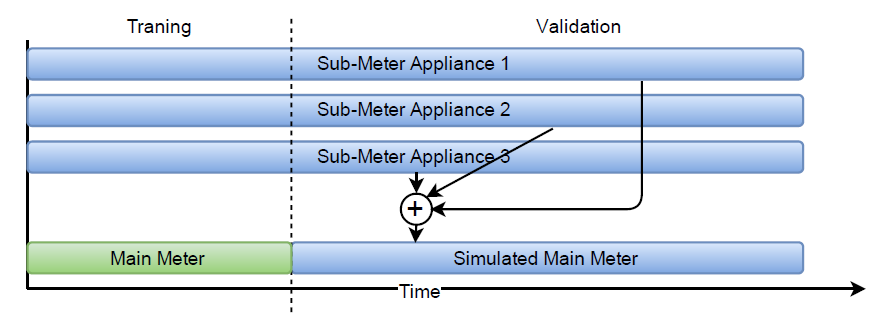
\includegraphics[width=1\textwidth]{billeder/REALSIM.png}
\caption{Illustration of dataset creation by combining real and constructed data}
\label{fig:REALSIMILU}
\end{figure}

In order to investigate these questions was a new dataset created that combined real data, collected from the house main meter, and an artificially constructed main meter. The new dataset was created by using the real data in the training period of the house, and using the constructed main meter in the validation, as illustrated on figure \ref{fig:REALSIMILU}.

This creates a very noisy environment in the training phase and a noise free environment in the validation phase. If the noise did not influence the creation of the statistical models that represent each appliance, then the results was expected to be just as good as for the noise free experiments conducted in section \ref{sec:NOISEFREE}.


\begin{table}[H]                             
\centering                                   
\begin{tabular}{cc|c|c|c|c|}
\cline{3-6}
\multicolumn{1}{l}{}                            &        & \multicolumn{2}{c|}{FHMM} & \multicolumn{2}{c|}{Parson} \\ \cline{3-6} 
\multicolumn{1}{l}{}                            &        & F1        & Accuracy      & F1         & Accuracy       \\ \hline
\multicolumn{1}{|c|}{\multirow{3}{*}{House 3}}  & TV 1   & 0.20      & 0.94          & 0.23       & 0.86           \\ \cline{2-6} 
\multicolumn{1}{|c|}{}                          & PC     & 0.29      & 0.94          & 0.32       & 0.92           \\ \cline{2-6} 
\multicolumn{1}{|c|}{}                          & TV 2   & 0.00      & 0.88          & 0.20       & 0.11           \\ \hline
\multicolumn{1}{|c|}{\multirow{4}{*}{House 10}} & TV 1   & 0.10      & 0.74          & 0.40       & 0.25           \\ \cline{2-6} 
\multicolumn{1}{|c|}{}                          & Stereo & -         & 1.00          & -          & 1.00           \\ \cline{2-6} 
\multicolumn{1}{|c|}{}                          & PC     & -         & 0.99          & -          & 0.99           \\ \cline{2-6} 
\multicolumn{1}{|c|}{}                          & TV 2   & -         & 0.99          & -          & 0.99           \\ \hline
\multicolumn{1}{|c|}{\multirow{3}{*}{House 18}} & TV 1   & 0.00      & 0.86          & 0.24       & 0.14           \\ \cline{2-6} 
\multicolumn{1}{|c|}{}                          & Lamp   & -         & 0.99          & -          & -              \\ \cline{2-6} 
\multicolumn{1}{|c|}{}                          & TV 2   & 0.73      & 0.58          & 0.73       & 0.58           \\ \hline
\end{tabular}                                
\caption{Disaggregation in real and constructed main meters combined.}                     
\label{table:Tab:SHGREALSIM}                 
\end{table}    

If the results from the experiment, shown in table \ref{table:Tab:SHGREALSIM} is compared with the results from table \ref{table:Tab:SHGSIM} from section \ref{sec:NOISEFREE} it is clearly seen that the performance of the system trained in real data is much lower than the one trained on only artificially constructed data. This indicates that the models obtained in the real data is influenced by the appliance noise, and is therefore not fitting accurately enough to the true appliance model. 

This could indicate that the low performance in the real data shown in table \ref{table:Tab:SHGREAL} in section \ref{sec:NOISE} is caused by the models not fitting correctly to the true values, and not by the models being triggered by application noise from other appliances.

In order to validate this hypothesis was a similar experiment conducted, where the training data was artificially constructed, and the validation data was the real data from the main meter as illustrated in figure \ref{fig:SHGSIMREAL}. 

\begin{figure}[H]
\centering
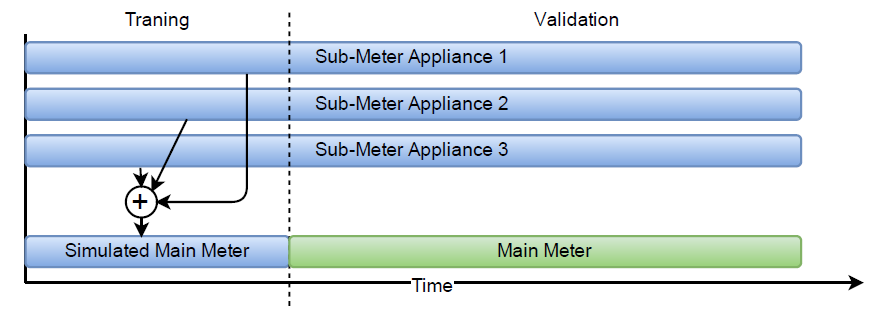
\includegraphics[width=0.9\textwidth]{billeder/SIMREAL.png}
\caption{Illustration of dataset creation by combining constructed and real data}
\label{fig:SHGSIMREAL}
\end{figure}

By training the model on the constructed data, is the true model for the appliances found. If the appliance noise in the real noisy environment is non-interfering can a performance like for the noise free environment described in section \ref{sec:NOISEFREE} be expected. 


\begin{table}[H]                             
\centering                                   
\begin{tabular}{lc|c|c|c|c|}
\cline{3-6}
                                                &        & \multicolumn{2}{c|}{FHMM} & \multicolumn{2}{c|}{Parson} \\ \cline{3-6} 
                                                &        & F1        & Accuracy      & F1         & Accuracy       \\ \hline
\multicolumn{1}{|l|}{\multirow{3}{*}{House 3}}  & TV 1   & 0.10      & 0.42          & 0.10       & 0.45           \\ \cline{2-6} 
\multicolumn{1}{|l|}{}                          & PC     & 0.13      & 0.39          & 0.12       & 0.44           \\ \cline{2-6} 
\multicolumn{1}{|l|}{}                          & TV 2   & 0.21      & 0.35          & 0.20       & 0.11           \\ \hline
\multicolumn{1}{|l|}{\multirow{4}{*}{House 10}} & TV 1   & 0.40      & 0.25          & 0.40       & 0.25           \\ \cline{2-6} 
\multicolumn{1}{|l|}{}                          & Stereo & -         & 1.00          & -          & 1.00           \\ \cline{2-6} 
\multicolumn{1}{|l|}{}                          & PC     & -         & 0.99          & -          & 0.99           \\ \cline{2-6} 
\multicolumn{1}{|l|}{}                          & TV 2   & -         & 0.99          & -          & 0.99           \\ \hline
\multicolumn{1}{|l|}{\multirow{3}{*}{House 18}} & TV 1   & 0.27      & 0.26          & 0.24       & 0.14           \\ \cline{2-6} 
\multicolumn{1}{|l|}{}                          & Lamp   & -         & 0.99          & -          & -              \\ \cline{2-6} 
\multicolumn{1}{|l|}{}                          & TV 2   & 0.73      & 0.58          & 0.73       & 0.58           \\ \hline
\end{tabular}                              
\caption{Disaggregation in constructed and real main meters combined}                     
\label{table:Tab:SHGSIMREAL}                 
\end{table}     

The results are shown in table \ref{table:Tab:SHGSIMREAL}. The performance of this system is lower than the one from the noise free experiment. This lead to the conclusion that the noise is both affecting the models, and interfering in the validation process.  

The results from the disaggregation of the data in the real environment from section \ref{sec:NOISE} is compared with the results from the the previous experiments, where the models was extracted from constructed data and validated on the real data, is shown in table \ref{table:Tab:RealVsCon}. 

\begin{table}[H]                             
\centering                                   
\begin{tabular}{ccccccc}
\cline{3-4} \cline{6-7}
\multicolumn{1}{l}{}                            & \multicolumn{1}{c|}{}       & \multicolumn{2}{c|}{FHMM}                                 & \multicolumn{1}{c|}{} & \multicolumn{2}{c|}{FHMM}                                 \\
\multicolumn{1}{l}{}                            & \multicolumn{1}{c|}{}       & \multicolumn{2}{c|}{Real}                                 & \multicolumn{1}{c|}{} & \multicolumn{2}{c|}{Constructed}                          \\ \cline{3-4} \cline{6-7} 
\multicolumn{1}{l}{}                            & \multicolumn{1}{c|}{}       & \multicolumn{1}{c|}{F1}   & \multicolumn{1}{c|}{Accuracy} & \multicolumn{1}{c|}{} & \multicolumn{1}{c|}{F1}   & \multicolumn{1}{c|}{Accuracy} \\ \cline{1-4} \cline{6-7} 
\multicolumn{1}{|c|}{\multirow{3}{*}{House 3}}  & \multicolumn{1}{c|}{TV 1}   & \multicolumn{1}{c|}{0.19} & \multicolumn{1}{c|}{0.74}     & \multicolumn{1}{c|}{} & \multicolumn{1}{c|}{0.10} & \multicolumn{1}{c|}{0.42}     \\ \cline{2-4} \cline{6-7} 
\multicolumn{1}{|c|}{}                          & \multicolumn{1}{c|}{PC}     & \multicolumn{1}{c|}{0.19} & \multicolumn{1}{c|}{0.84}     & \multicolumn{1}{c|}{} & \multicolumn{1}{c|}{0.13} & \multicolumn{1}{c|}{0.39}     \\ \cline{2-4} \cline{6-7} 
\multicolumn{1}{|c|}{}                          & \multicolumn{1}{c|}{TV 2}   & \multicolumn{1}{c|}{0.03} & \multicolumn{1}{c|}{0.84}     & \multicolumn{1}{c|}{} & \multicolumn{1}{c|}{0.21} & \multicolumn{1}{c|}{0.35}     \\ \cline{1-4} \cline{6-7} 
\multicolumn{1}{l}{}                            &                             &                           &                               &                       &                           &                               \\ \cline{1-4} \cline{6-7} 
\multicolumn{1}{|c|}{\multirow{4}{*}{House 10}} & \multicolumn{1}{c|}{TV 1}   & \multicolumn{1}{c|}{0.60} & \multicolumn{1}{c|}{0.76}     & \multicolumn{1}{c|}{} & \multicolumn{1}{c|}{0.40} & \multicolumn{1}{c|}{0.25}     \\ \cline{2-4} \cline{6-7} 
\multicolumn{1}{|c|}{}                          & \multicolumn{1}{c|}{Stereo} & \multicolumn{1}{c|}{-}    & \multicolumn{1}{c|}{1.00}     & \multicolumn{1}{c|}{} & \multicolumn{1}{c|}{-}    & \multicolumn{1}{c|}{1.00}     \\ \cline{2-4} \cline{6-7} 
\multicolumn{1}{|c|}{}                          & \multicolumn{1}{c|}{PC}     & \multicolumn{1}{c|}{-}    & \multicolumn{1}{c|}{0.99}     & \multicolumn{1}{c|}{} & \multicolumn{1}{c|}{-}    & \multicolumn{1}{c|}{0.99}     \\ \cline{2-4} \cline{6-7} 
\multicolumn{1}{|c|}{}                          & \multicolumn{1}{c|}{TV 2}   & \multicolumn{1}{c|}{-}    & \multicolumn{1}{c|}{0.99}     & \multicolumn{1}{c|}{} & \multicolumn{1}{c|}{-}    & \multicolumn{1}{c|}{0.99}     \\ \cline{1-4} \cline{6-7} 
\multicolumn{1}{l}{}                            &                             &                           &                               &                       &                           &                               \\ \cline{1-4} \cline{6-7} 
\multicolumn{1}{|c|}{\multirow{3}{*}{House 18}} & \multicolumn{1}{c|}{TV 1}   & \multicolumn{1}{c|}{0.36} & \multicolumn{1}{c|}{0.65}     & \multicolumn{1}{c|}{} & \multicolumn{1}{c|}{0.27} & \multicolumn{1}{c|}{0.26}     \\ \cline{2-4} \cline{6-7} 
\multicolumn{1}{|c|}{}                          & \multicolumn{1}{c|}{Lamp}   & \multicolumn{1}{c|}{-}    & \multicolumn{1}{c|}{0.99}     & \multicolumn{1}{c|}{} & \multicolumn{1}{c|}{-}    & \multicolumn{1}{c|}{0.99}     \\ \cline{2-4} \cline{6-7} 
\multicolumn{1}{|c|}{}                          & \multicolumn{1}{c|}{TV 2}   & \multicolumn{1}{c|}{0.73} & \multicolumn{1}{c|}{0.58}     & \multicolumn{1}{c|}{} & \multicolumn{1}{c|}{0.73} & \multicolumn{1}{c|}{0.58}     \\ \cline{1-4} \cline{6-7} 
\end{tabular}                         
\caption{Trained in real vs. constructed data}                     
\label{table:Tab:RealVsCon}                    
\end{table}  

The table shows that the performance of the system is better when trained in the real environment, as in relation to when the the system is trained in a noise free environment and then deployed in a noisy environment. This is in contrast to what one might think, since the noise free environment should have supplied more correct models. But when the appliance noise is removed from a house, in the training process, is a bias error introduced. 

Appliances such as refrigerators and freezers that are always on will create a local house bias. This will vary from house to house, and is depended on the types and number of appliances in the house. If only a small number of devices are modelled in each house, as in the SmartHG case, is the bias almost exclusivity a part of the appliance noise. When the models are fitted by training in the real data, is the bias learned into the model, and further improves the model. This is not the case when the model are trained in the constructed dataset. 

If not all appliances in a house is known, a better performance can therefore be obtained by training in the intended environment of deployment. 

Some algorithms are designed to not be affected by the house bias, and is therefore moved from different environments more easily. The Parson algorithm is designed with this in mind. The performance of the parson algorithm is therefore the same, or in some cases improved, when using models trained in constructed data. This advantage unfortunately comes with the problem of generalization, which lead to harder source separation, as discussed in section \ref{sec:NOISE}. 


\section{Model Size And Completeness Influence }
Some of the parameters that often differ in the many different environments \ab{NILM} applications are deployed in, is the number of appliances in the environment, and the number of appliances that are known in the environment.  

The environment size or complexity is a parameter that tells how many devices that are in a given environment. As the complexity in a \ab{NILM} application is increasing the detection rate is deceasing\citep{RefWorks:34}. This is one of the major problems and is why many researchers only focus on a small subset of appliances that have a fairly unique consumption signature. 

The model completeness is a metric describing how many appliances are known by the application in relation to the total amount of appliances. This can also be seen as the amount of appliance noise as discussed in section \ref{sec:AppNoise}.

\subsection{Test Set Creation}
\label{sec:datasetCreation}
In order to experiment with the completeness and complexity in the SmartHG dataset is a more controllable series of datasets artificially constructed from the SmartHG dataset. 

First an artificial house where created called the "TV House" dataset. The TV house dataset is created by picking the relative dominant TV signals from the houses 5,10,11,13,18 and 23 in the SmartHG dataset and combining them to one artificial house with 7 TV's. 

This dataset contains of dominant appliances, and there is no appliance noise from unknown devices. It is still worth noticing that all the 7 appliances are a Type-II appliances, and they are all TV's, which make there usage pattern some what similar. Since the Parson algorithm is greatly effected by this will the focus mainly be on the \ab{FHMM} algorithm. 

If the TV House dataset was seen as a set of sub-meters as mathematically shown in equation \ref{EQ:SUBMS}. 

\begin{equation}
	H_{full} = \{ TV_1, TV_2, ... , TV_7 \}
	\label{EQ:SUBMS}
\end{equation}

Since there is no appliance noise, can the main meter data be found as the sum of sub-meters data as shown in equation \ref{EQ:SUMSUB}. 

\begin{equation}
	M_{main} = \sum_{X \in H_{full}}X
	\label{EQ:SUMSUB}
\end{equation}

Using this information it is possible to create a set with a specified complexity, by taking a subset of the $H_{full}$ set with the cardinality of the specified complexity. The main meter can now be found on this subset using the same principle as in equation \ref{EQ:SUMSUB}. Using the equation \ref{EQ:TVCARSET}, it is possible to find a set of all sets with a desired complexity $c$.

\begin{equation}
	\textbf{H}_c = \{ x | x \in \powerset{H_{full}}, \forall |x| = c   \}
	\label{EQ:TVCARSET}
\end{equation}

This can be graphically shown as in figure \ref{fig:PSILLU}. 

\begin{figure}[H]
\begin{picture}(0,200)
\put(0,0){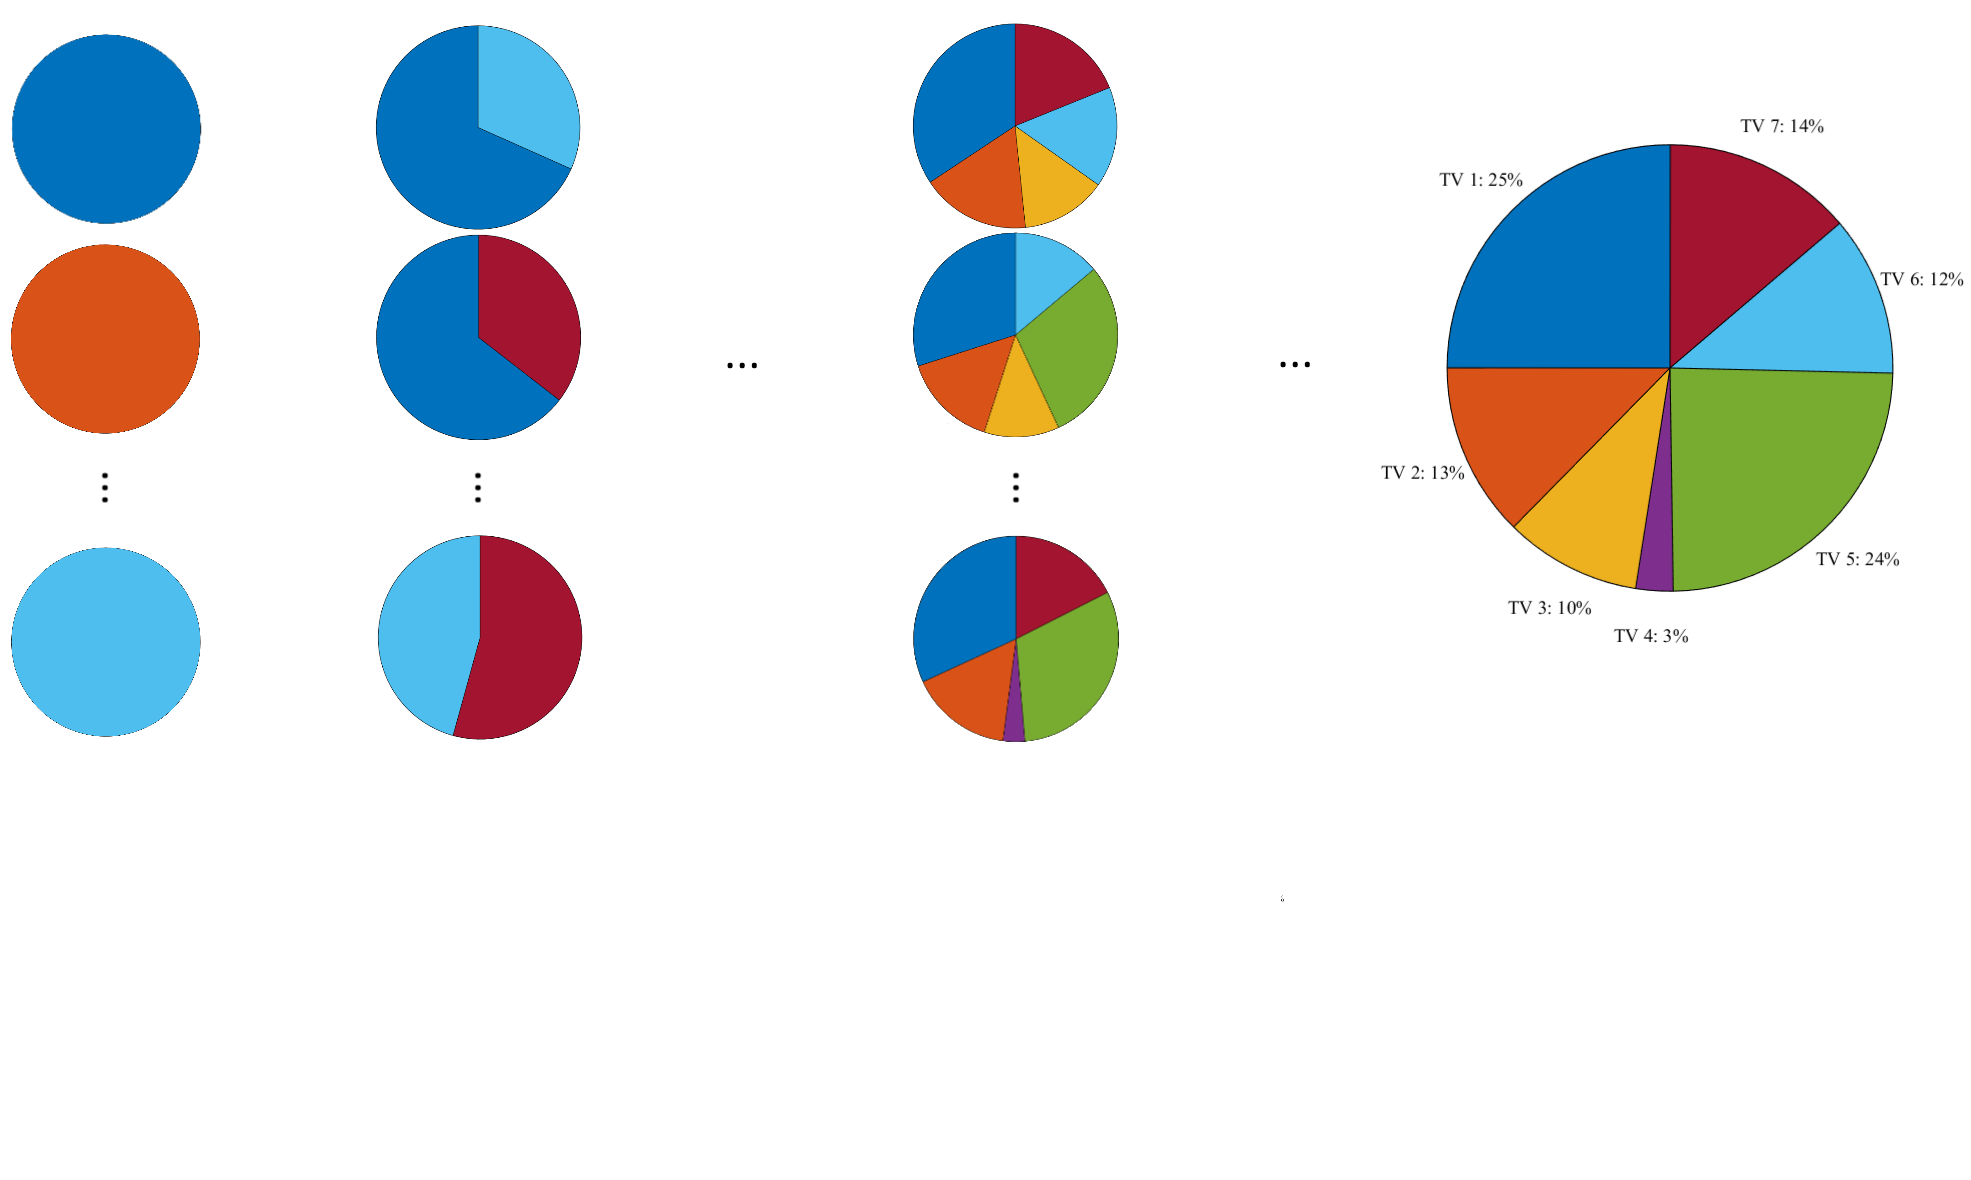
\includegraphics[width=1\textwidth]{billeder/CombiShow.png}}

\put(20,10){$\textbf{H}_1$}
\put(105,10){$\textbf{H}_2$}
\put(230,10){$\textbf{H}_5$}
\put(375,10){$\textbf{H}_7$}

\end{picture}
\caption{$\textbf{H}_c$ sets from the TV house dataset}
\label{fig:PSILLU}
\end{figure}

Where the $\textbf{H}_7$ only contains the $H_{full}$ set. In this manner it is possible to artificially create one or more datasets in a desired complexity equal to or less than the $H_{full}$ complexity. The amount of artificiality created houses for a given complexity can be found by using the simple combinatorial equation shown in equation \ref{EQ:nCr}.

\begin{gather}
		|\textbf{H}_c| = \frac{|H_{full}|!}{c! \times (|H_{full}| - c)!} \label{EQ:nCr} \\
		A_c = |\textbf{H}_c| \times \frac{c}{|H_{full}|} \label{EQ:ACr}
\end{gather}
% n! / ( r! (n - r)! )


As illustrated on figure \ref{fig:PSILLU} can an appliance appear in multiple sets in a given $\textbf{H}_c$ collection. The number of sets containing a specific appliance in a $\textbf{H}_c$ collection $A_c$ can be calculated as in equation \ref{EQ:ACr}. In order to ensure that the combination of appliances does not have an effect on the experiments, are the experiments conducted on all combinations in $\textbf{H}_c$. The results for each experiment is an average of the performance for the appliance in the experiment. 

\begin{table}[]
\centering
\begin{tabular}{c|c|c|c|c|c|c|c|}
\cline{2-8}
                       & $c = 1$ & $c = 2$ & $c = 3$ & $c = 4$ & $c = 5$ & $c = 6$ & $c = 7$ \\ \hline
\multicolumn{1}{|c|}{$|\textbf{H}_c|$} &    7   &    21   &    35   &    35   &   21    &   7    &    1  \\ \hline
\multicolumn{1}{|c|}{$A_c$} &    1   &     6  &     15  &     20  &    15   &    6   &    1   \\ \hline
\end{tabular}
\caption{TV House dataset complexity}
\label{Tab:TvHouse}
\end{table}

In the case of the TV house dataset can the $|\textbf{H}_c|$ and $A_c$ values for the different complexity be seen in table \ref{Tab:TvHouse}.


\subsection{Model Complexity Test}
\label{sec:MCT}
To investigate the effect the number of appliances in a house, have on the performance of a \ab{NILM} system, is disaggregation done on every artificial house in $\textbf{H}$.

\begin{figure}[H]
\centering
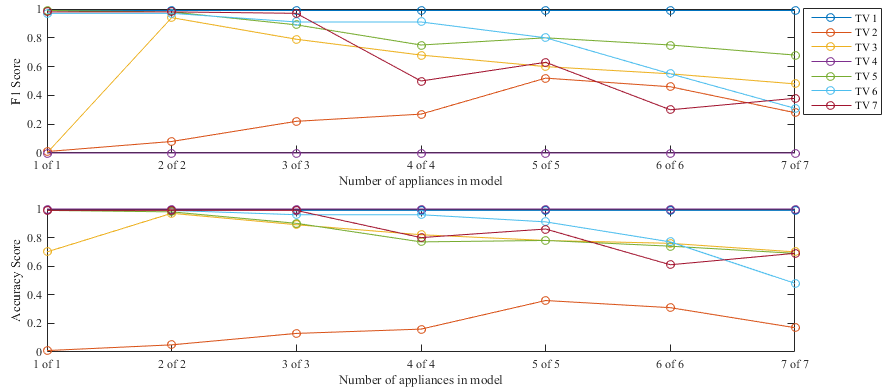
\includegraphics[width=1\textwidth]{billeder/ModelSize.png}
\caption{Average score at different complexity }
\label{fig:COMPT}
\end{figure}

The test is preformed on every combination, to ensure that there is not some combination that are more favourable than others. The results shown in figure \ref{fig:COMPT} are the average of the results from the many combinations as described in section \ref{sec:datasetCreation}. 

For the most part it is fairly easy to correctly classify the TV's when the complexity is only one. As a general trend does the F1 and accuracy score of the TV's decrees as the complexity of the house increase. This is due to the application spill over effect. The spill over effect is when there actually is an event, but the system classifies it to the wrong device.  An effect of this is most clearly seen on TV 2 signal. TV 2 is a very complex signal, and is therefore hard to track by the algorithm, as seen at the $\textbf{H}_1$ complexity that have a F1 score on almost zero. When the complexity is increased it looks like it is easier to detect the signal, and the F1 score is increasing. What is actually happening is the spill effect from the other TV's. Since all the appliances are TV's they have a lot of overlap in their usage. A lot of people watches TV at the same time of day e.g. between 18-22. This makes the algorithm encounter signal's that are similar in structure for the different TV's, and it have a hard time deciding which appliance is responsible. Therefore can some of the events generated by the other TV's spill over in TV 2. If by chance TV 2 actually was on when the events from the other TV's was wrongfully assigned, the F1 and accuracy score of TV 2 would improve. 

For other appliances that are not as hard to classify as TV 2 will the spill over effect decrease the F1 and accuracy score as seen on the figure. 

\subsection{Model Completeness Influence }
In the experiments conducted on the the SmartHG dataset in section \ref{sec:AppNoise} it was shown that the appliance noise made it hard to correctly disaggregate the appliances of the houses. In the last experiment in section \ref{sec:MCT}, it was shown that the performance of the disaggregation was higher when the complexity of the house was low. This is much the same results as seen in the experiments on the SmartHG dataset, where the completely simulated house, that had a low complexity, preformed better than the real house with a high complexity. 

But in the SmartHG dataset was the complexity of the real dataset unknown since the amount of appliances that generated the appliance noise is unknown. It is therefore hard to conclude if the poor performance in the real data is due to the fact that the appliances is unknown by the disaggregation model, or because the complexity of the house is greater for the real data. 

To further investigate this was an experiment conducted on the TV house dataset, where the house models where trained on the $\textbf{H}_{7}$ dataset. The models trained did not contain the full knowledge of the house. The models was only trained to find a subset of meters in the house. Like for the experiments in section \ref{sec:MCT}, was the experiment conducted on all subset combinations. 

\begin{figure}[H]
\centering
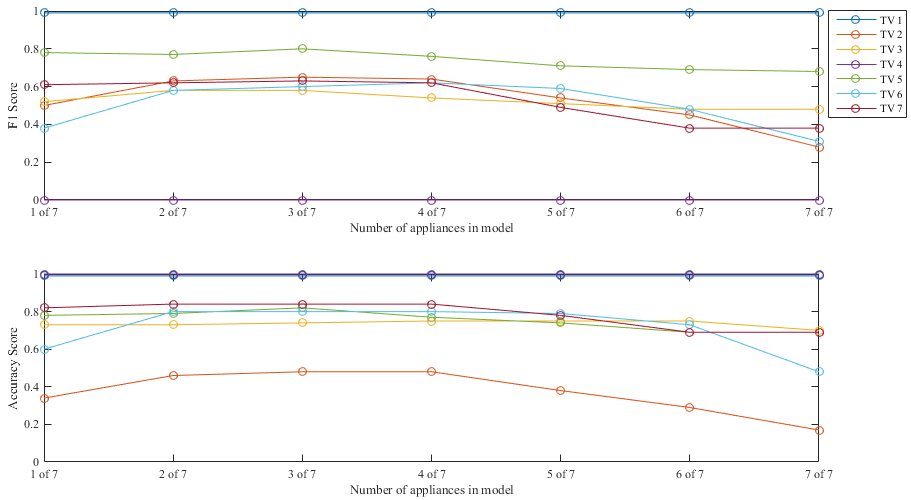
\includegraphics[width=1\textwidth]{billeder/ModelCompletness.png}
\caption{Completeness test of disaggregation of appliances in the TV house dataset }
\label{fig:COD}
\end{figure}

In figure \ref{fig:COD} is the result for each appliance shown. The result is an average of all tests at a given model completeness. It is seen from the figure that even though the disaggregation algorithm obtains more information about the complete house, it does not improve the recondition. 

This indicates that the 7 algorithms working in parallel, each disaggregating one meter, would obtain the same results as one model capable of seeing the house as a hole. It is worth mentioning that these tests are based on the \ab{FHMM} algorithm and other algorithms might preform different in this aspect. 

The results indicate that the complexity of the house is a more determining factor for the performance than the completeness of the model. 

\section{Chapter Discussion}
The findings in this chapter indicates that the complexity of a dataset have a profound impact on the detection performance. A simple way to decrease the performance in a house is to look at each phase in the house separately. This is one of the techniques used in the \ab{ECO} dataset to improve the performance in the system. This does require additional knowledge of which appliances that are connected to which phases. This knowledge can be analytical extracted from the dataset, or must be supplied at training time. 

It is also indicated that the methods based on the \ab{HMM} does not greatly improve by knowing the entire house model, in relation to only knowing a sub part. This can indicate that a system that focus on detecting each appliance individuality, potentially can detect the appliance as well as one that tires to see the house as a hole.   

The many problems that can occur when using small consumers and once that are similar in behaviour is nicely illustrated in the chapter. The spill over effect for similar appliances is greatly decreasing the overall performance, and the small consumers is almost undetectable. In order to better this performance, more unique features is needed. This could either be higher frequency features, as discussed in chapter \ref{sec:AppRec}, or by using reactive features. Furthermore it is shown that the best performance is obtained by training in the same environment as the solution will be deployed in. This is a subject that is also discussed by the developers of the Parson and Weiss algorithms \citep{RefWorks:28} \citep{RefWorks:23}, where they discussed ways to train or fit the models to the desired deployment environment.  

%4 pages
\glsresetall
\chapter{NILM As An Application} 
\label{sec:CaseStudy}
The last couple of years have the number of smart meters installed in residential houses increased drastically~\citep{RefWorks:44},~\citep{RefWorks:45}. The motivation for installing smart meters in the different houses have been to better understand energy consumption, in order to better plan energy distribution and production, and increase security~\citep{RefWorks:43}. This on of steps in creating a modern smart grid. With the smart grid came an opportunity for \ab{NILM}, since the equipment and infrastructure needed to measure the consumption and transfer the results through the Internet will be available in many households. 

The applications proposed in many of the articles published about \ab{NILM} focuses on energy management. Either it is for the electricity producers, that needs it to better predict consump-tion, or it is for the resident of the house that can optimize power usage to obtain savings \citep{RefWorks:17}. Even though these are fine examples of the potential usages of \ab{NILM} there might also exist an opportunity for the \dfs{service provider} in the smart grid to sell the \ab{NILM} information. An instance that collect information with the purpose of selling it is defined as a \df{data broker}. This chapter contains a small case study to illustrate how a \df{service provider} could obtain TV information from a city and act as a \df{data broker} to a local TV station. 

\section{The TV Viewing Habits Case}
The case setting is a small town, which have a number of households and an electricity utility company supplying energy to the city. For this case data from the SmartHG dataset is used to simulate a small town with 4 houses. The houses selected for this case are 10, 13, 18 and 23  since they contain a TV that are relatively dominant, as discussed in Section~\ref{sec:MMIRTSM}. 

\begin{figure}[H]
\begin{picture}(0,150)
\put(100,0){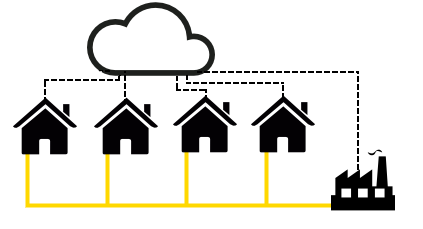
\includegraphics[width=0.6\textwidth]{billeder/CaseIlu.png}}

\put(177,110){Network}
\put(316,85){Service}
\put(312,75){Provider}

\put(319,0){Utility}
\put(314,-10){Company}

\put(122,62){\color{white} \textbf{10}}
\put(174,62){\color{white} \textbf{13}}
\put(226,62){\color{white} \textbf{18}}
\put(276,62){\color{white} \textbf{23}}
\put(200,0){Power Line}

\end{picture}
\caption{The city setup}
\label{fig:CaseSetup}
\end{figure}

The city setup is illustrated in Figure~\ref{fig:CaseSetup}. The figure illustrates how the utility company have a \df{generator} role and supplies energy to the houses. All the houses have smart meters, and are informing the utility company and the \dfs{service provider} about the current consumption of each house. This is done using some network. This is a fairly simplified example of a smart grid, where only the \df{customer}, \df{generator} and \df{service provider} roles are used. The power line is illustrated as a single feeder, but could just as well be a complex \df{distribution} network. In this case is it assumed that the \df{customer} sends information about the consumption of the houses every 30 seconds, as in the SmartHG dataset. Even though many smart meters today are capable of delivering information at this speed, it is more common to only get information each hour. This is mainly because the information is used to regulate distribution and production, which is a slow process that would not improve by faster update rates.  

The \dfs{service provider} collect the information from the smart meters, and by using \ab{NILM} can calculate statistical information about the town. In the fictive case is a local TV station interested in knowing what time a day the citizens of the town watches TV, in order to improve some aspect of their product. 

\section{Methodology}
The aim of this case is to illustrate the potential of this kind of application for a \df{service provider}. Therefore is the data analysis conducted in a manner, that illustrates how a \df{service provider} could do it. This means that only the main meter information is used in the analysis, and the sub-meter information is only used to validate the results.  The goal is for the \df{service provider} to disaggregate the TV signals from the main meter signal, in order to use it in some statistical analysis. 

\begin{figure}[H]
\centering
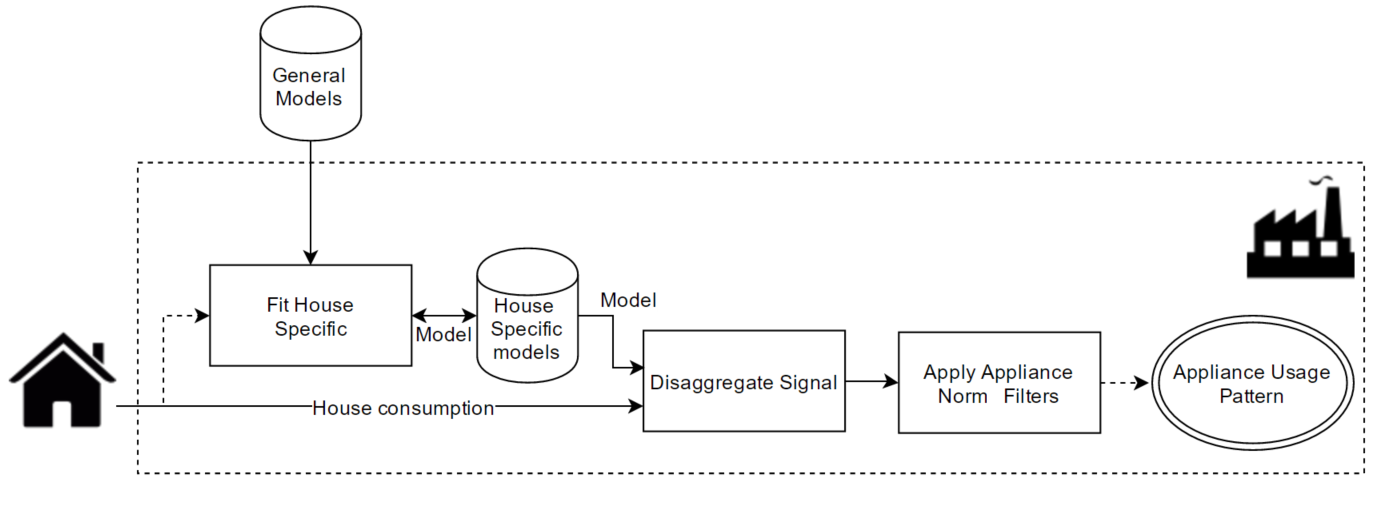
\includegraphics[width=1\textwidth]{billeder/Electric company method.png}
\caption{The disaggregation process}
\label{fig:ECM}
\end{figure}

This process is illustrated in Figure~\ref{fig:ECM}. It is assumed that the \dfs{service provider} have access to a very general statistical model of the TV. This model can come from some outside database, or be one that the utility company or \df{service provider} developed themselves. The first step is to create a household specific model, which is a specialisation of the general model. This could be done with sub-meter data. To make the experiment more realistic is the training of the statistical disaggregation models done using only the accumulated data from the main meter. This is done using the same method as developed for the Parson algorithm \citep{RefWorks:28}. This method finds periods where an appliance is turned ON and OFF without any other appliances changing states, is detected. These ON/OFF single-event fragments are then mapped to specific appliances using the general models. When enough ON/OFF single-event fragments have been collected, can this information be used to train a more specific model. This can happen in a contentiously manner where the specific model is improved as more data is collected.  

Using the specific models can disaggregation of the main meter signal be achieved. The statistical disaggregation models selected in this case are found using the \ab{FHMM} algorithm. As discussed in Section~\ref{sec:NOISE}, the disaggregation alone gives a very error prone signal. The signal is therefore feed through a \df{norm filter}. As discussed in Section~\ref{sec:NormFilter} can the information about how a user normally would use the appliance be used to filter the disaggregated data to obtain better results. 

The result of this process is an appliance usage pattern, that can be used by the \dfs{service provider} to derive various statistical properties.  

The experiment is conducted with four weeks of data been used to train TV specific models for each house. The analysis for the TV station is conducted over a period of six weeks that is not overlapping with the initial four training weeks. 

\section{Results}
The viewing habits of the small town obtained by the disaggregation analysis is compared with the actual viewing habit obtained from the sub-meter data. In Figure~\ref{fig:WHW} is the results shown for the first week. Plots showing the disaggregation of the entire period for each appliance can be found in Appendix~\ref{APP:viewship}.

\begin{figure}[H]
\centering
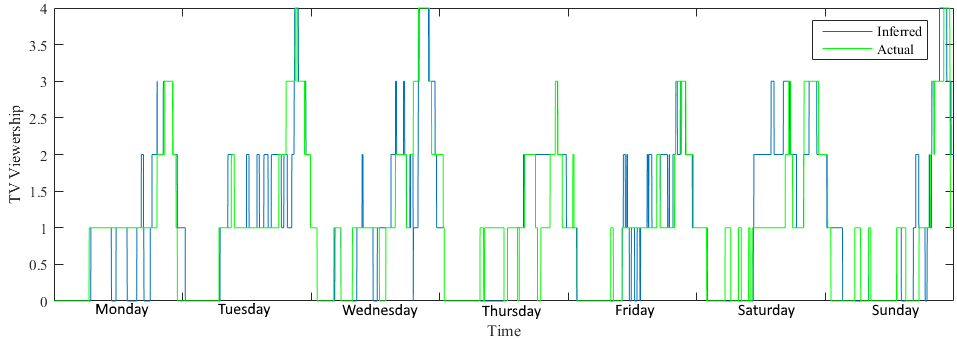
\includegraphics[width=1\textwidth]{billeder/Viewership.png}
\caption{Viewership in week one}
\label{fig:WHW}
\end{figure}

The figure shows the viewership, that tells how many in the city is watching TV at a given time. The green line is the actual viewership, where the blue is the viewership reported by the utility company. The results differed, as one would expect, since the disaggregation process in an environment with high \df{background consumption} is a hard task. The general trends that many are watching TV in the evening, and not that many in the morning, is still represented nicely. This illustrates that the general trends of the viewership is maintained in the disaggregated signal, and this is commonly what is important for this kind of costumer statistics. 

In Table~\ref{tab:CaseRes} is the average number of viewers in 3 hour timeslots shown. The results shown in the table is the average of all 6 weeks, split up in the different weekdays. 

% Please add the following required packages to your document preamble:
% \usepackage{multirow}
\begin{table}[H]
\centering
\begin{tabular}{lccccccccc}
\cline{3-10}
                                                & \multicolumn{1}{c|}{}         & \multicolumn{8}{c|}{Time of day}                                                                                                                                                                                                                                                                              \\ \cline{3-10} 
                                                & \multicolumn{1}{c|}{}         & \multicolumn{1}{c|}{\textbf{00-03}} & \multicolumn{1}{c|}{\textbf{03-06}} & \multicolumn{1}{c|}{\textbf{06-09}} & \multicolumn{1}{c|}{\textbf{09-12}} & \multicolumn{1}{c|}{\textbf{12-13}} & \multicolumn{1}{c|}{\textbf{15-18}} & \multicolumn{1}{c|}{\textbf{18-21}} & \multicolumn{1}{c|}{\textbf{21-00}} \\ \cline{3-10} 
                                                &                               &                                     &                                     &                                     &                                     &                                     &                                     &                                     &                                     \\ \cline{2-10} 
\multicolumn{1}{l|}{\multirow{2}{*}{Monday}}    & \multicolumn{1}{c|}{Inferred} & \multicolumn{1}{c|}{0.12}           & \multicolumn{1}{c|}{0.00}           & \multicolumn{1}{c|}{0.66}           & \multicolumn{1}{c|}{1.19}           & \multicolumn{1}{c|}{1.02}           & \multicolumn{1}{c|}{1.31}           & \multicolumn{1}{c|}{2.39}           & \multicolumn{1}{c|}{2.08}           \\ \cline{2-10} 
\multicolumn{1}{l|}{}                           & \multicolumn{1}{c|}{True}     & \multicolumn{1}{c|}{0.13}           & \multicolumn{1}{c|}{0.28}           & \multicolumn{1}{c|}{0.98}           & \multicolumn{1}{c|}{0.87}           & \multicolumn{1}{c|}{0.68}           & \multicolumn{1}{c|}{1.28}           & \multicolumn{1}{c|}{2.49}           & \multicolumn{1}{c|}{1.72}           \\ \cline{2-10} 
                                                &                               &                                     &                                     &                                     &                                     &                                     &                                     &                                     &                                     \\ \cline{2-10} 
\multicolumn{1}{l|}{\multirow{2}{*}{Tuesday}}   & \multicolumn{1}{c|}{Inferred} & \multicolumn{1}{c|}{0.13}           & \multicolumn{1}{c|}{0.28}           & \multicolumn{1}{c|}{0.98}           & \multicolumn{1}{c|}{0.87}           & \multicolumn{1}{c|}{0.68}           & \multicolumn{1}{c|}{1.28}           & \multicolumn{1}{c|}{2.49}           & \multicolumn{1}{c|}{1.72}           \\ \cline{2-10} 
\multicolumn{1}{l|}{}                           & \multicolumn{1}{c|}{True}     & \multicolumn{1}{c|}{0.19}           & \multicolumn{1}{c|}{0.09}           & \multicolumn{1}{c|}{0.39}           & \multicolumn{1}{c|}{0.88}           & \multicolumn{1}{c|}{0.73}           & \multicolumn{1}{c|}{1.24}           & \multicolumn{1}{c|}{2.23}           & \multicolumn{1}{c|}{2.26}           \\ \cline{2-10} 
                                                &                               &                                     &                                     &                                     &                                     &                                     &                                     &                                     &                                     \\ \cline{2-10} 
\multicolumn{1}{l|}{\multirow{2}{*}{Wednesday}} & \multicolumn{1}{c|}{Inferred} & \multicolumn{1}{c|}{0.19}           & \multicolumn{1}{c|}{0.09}           & \multicolumn{1}{c|}{0.39}           & \multicolumn{1}{c|}{0.88}           & \multicolumn{1}{c|}{0.73}           & \multicolumn{1}{c|}{1.24}           & \multicolumn{1}{c|}{2.23}           & \multicolumn{1}{c|}{2.26}           \\ \cline{2-10} 
\multicolumn{1}{l|}{}                           & \multicolumn{1}{c|}{True}     & \multicolumn{1}{c|}{0.09}           & \multicolumn{1}{c|}{0.30}           & \multicolumn{1}{c|}{0.58}           & \multicolumn{1}{c|}{0.79}           & \multicolumn{1}{c|}{0.77}           & \multicolumn{1}{c|}{1.42}           & \multicolumn{1}{c|}{2.72}           & \multicolumn{1}{c|}{2.11}           \\ \cline{2-10} 
\multicolumn{1}{c}{}                            &                               &                                     &                                     &                                     &                                     &                                     &                                     &                                     &                                     \\ \cline{2-10} 
\multicolumn{1}{l|}{\multirow{2}{*}{Thursday}}  & \multicolumn{1}{c|}{Inferred} & \multicolumn{1}{c|}{0.09}           & \multicolumn{1}{c|}{0.30}           & \multicolumn{1}{c|}{0.58}           & \multicolumn{1}{c|}{0.79}           & \multicolumn{1}{c|}{0.77}           & \multicolumn{1}{c|}{1.42}           & \multicolumn{1}{c|}{2.72}           & \multicolumn{1}{c|}{2.11}           \\ \cline{2-10} 
\multicolumn{1}{l|}{}                           & \multicolumn{1}{c|}{True}     & \multicolumn{1}{c|}{0.12}           & \multicolumn{1}{c|}{0.09}           & \multicolumn{1}{c|}{0.31}           & \multicolumn{1}{c|}{0.96}           & \multicolumn{1}{c|}{1.12}           & \multicolumn{1}{c|}{1.69}           & \multicolumn{1}{c|}{2.86}           & \multicolumn{1}{c|}{2.30}           \\ \cline{2-10} 
                                                &                               &                                     &                                     &                                     &                                     &                                     &                                     &                                     &                                     \\ \cline{2-10} 
\multicolumn{1}{l|}{\multirow{2}{*}{Friday}}    & \multicolumn{1}{c|}{Inferred} & \multicolumn{1}{c|}{0.12}           & \multicolumn{1}{c|}{0.09}           & \multicolumn{1}{c|}{0.31}           & \multicolumn{1}{c|}{0.96}           & \multicolumn{1}{c|}{1.12}           & \multicolumn{1}{c|}{1.69}           & \multicolumn{1}{c|}{2.86}           & \multicolumn{1}{c|}{2.30}           \\ \cline{2-10} 
\multicolumn{1}{l|}{}                           & \multicolumn{1}{c|}{True}     & \multicolumn{1}{c|}{0.10}           & \multicolumn{1}{c|}{0.18}           & \multicolumn{1}{c|}{0.66}           & \multicolumn{1}{c|}{0.91}           & \multicolumn{1}{c|}{0.74}           & \multicolumn{1}{c|}{1.65}           & \multicolumn{1}{c|}{3.17}           & \multicolumn{1}{c|}{2.35}           \\ \cline{2-10} 
                                                &                               &                                     &                                     &                                     &                                     &                                     &                                     &                                     &                                     \\ \cline{2-10} 
\multicolumn{1}{l|}{\multirow{2}{*}{Saturday}}  & \multicolumn{1}{c|}{Inferred} & \multicolumn{1}{c|}{0.10}           & \multicolumn{1}{c|}{0.18}           & \multicolumn{1}{c|}{0.66}           & \multicolumn{1}{c|}{0.91}           & \multicolumn{1}{c|}{0.74}           & \multicolumn{1}{c|}{1.65}           & \multicolumn{1}{c|}{3.17}           & \multicolumn{1}{c|}{2.35}           \\ \cline{2-10} 
\multicolumn{1}{l|}{}                           & \multicolumn{1}{c|}{True}     & \multicolumn{1}{c|}{0.28}           & \multicolumn{1}{c|}{0.17}           & \multicolumn{1}{c|}{0.95}           & \multicolumn{1}{c|}{0.77}           & \multicolumn{1}{c|}{1.39}           & \multicolumn{1}{c|}{1.36}           & \multicolumn{1}{c|}{2.26}           & \multicolumn{1}{c|}{2.10}           \\ \cline{2-10} 
                                                &                               &                                     &                                     &                                     &                                     &                                     &                                     &                                     &                                     \\ \cline{2-10} 
\multicolumn{1}{l|}{\multirow{2}{*}{Sunday}}    & \multicolumn{1}{c|}{Inferred} & \multicolumn{1}{c|}{0.28}           & \multicolumn{1}{c|}{0.17}           & \multicolumn{1}{c|}{0.95}           & \multicolumn{1}{c|}{0.77}           & \multicolumn{1}{c|}{1.39}           & \multicolumn{1}{c|}{1.36}           & \multicolumn{1}{c|}{2.26}           & \multicolumn{1}{c|}{2.10}           \\ \cline{2-10} 
\multicolumn{1}{l|}{}                           & \multicolumn{1}{c|}{True}     & \multicolumn{1}{c|}{0.12}           & \multicolumn{1}{c|}{0.00}           & \multicolumn{1}{c|}{1.01}           & \multicolumn{1}{c|}{0.96}           & \multicolumn{1}{c|}{0.96}           & \multicolumn{1}{c|}{1.33}           & \multicolumn{1}{c|}{1.93}           & \multicolumn{1}{c|}{1.65}           \\ \cline{2-10} 
\end{tabular}
\caption{Average viewership in a 6 week period.}
\label{tab:CaseRes}
\end{table}

This illustrates that the true trends in the information is maintained. The results indicates that it is to some degree possible to obtain user information from the disaggregated data. The TV is a relative hard appliance to detect, since there are many different types. The success in this experiment is partly due to the fact that the TV was some of the main consumers of the houses selected, and they had a pure Type-I behaviour.

At the current state of \ab{NILM} is the information only limited to a small amount of devices, since it is hard to detect other appliances than the top consumers in a household. One of the techniques shown to greatly improve the effectiveness of \ab{NILM} is to switch from the sub 1 Hz sampling range to a higher sampling rate in the kHz range. In the future there might be smart meters capable of delivering information at high frequency or the \ab{NILM} techniques have advanced so it is possible to detect all appliances. This will greatly improve the possibility for the \dfs{service provider} to deliver very detailed user behavioural statistics. This information can be of interest for companies developing and selling electronics, since they are able to get accurate user reports about their products. 

\section{Chapter Summery}
This case is a very simple example of how the \dfs{service provider} can extend their product range to statistical information. This information could potentially also be used to extend their product range to the \dfs{customer}. One example of this could be a fridge surveillance system that would send warning messages to the resident if their fridge stopped working.

The cases focused around getting information from a TV. This information was used to extract some general statistical properties about a small city's viewing habits. This is done by using the \ab{FHMM} algorithm and a \df{norm filter}. The approach is relatively successful. This indicates that such approaches can be used to extend the \dfs{service provider} product range. All TV appliances was relatively large energy consumers in the house. This makes them easy to detect. For appliances that are small consumers it is unlikely that the approach will have as big an effect.

% 3 pages
\glsresetall
\chapter{Discussion}

\Ab{NILM} is an area of research that is gaining a lot of attention due to the more complex smart grid structures. Some of the challenges in the smart grid is that there is not just one producer and a series of consumers. There can be multiple of both, and some households contains solar panels, or other energy producing technologies, that makes them bout producer and consumer at different times. This creates challenges for some of the \ab{NILM} applications, as it can camouflage the true power consumption of the houses. The same problem can be created by battery devices, that can mask the a appliance power demand. Some of these problems can be observed by monitoring the data quality.

\section{Creating High Quality Measurements}
When monitoring the the data quality as in chapter \ref{Sec:DataQuality} a range of problems when collecting consumption data can be detected. When observing the collection of SmartHG data there were two error gropes that reviled itself. The one was equipment failure. Both failure for a specific meter, or the server was detected. The second is the houses that exhibit masking behaviour. By looking at the information collected by the sub-meters and comparing it with the main meter data it is possible to detect the masking behaviour created by devices such as solar cells or backup batteries. 

By detecting the errors during the measurement period it is possible to correct the errors. This creates better and more clean measurements. By looking at the measurements activity, it is possible to find still and active areas. This can be used to find active and inactive periods of the devices. These periods can be used to create a more direct training of the statistical models used to do appliance disaggregation. Finding periods in the data where only one single appliance have a ON/OFF cycle, without any other appliance changes state, have shown to be an important training technique. This technique is mostly relevant if sub-meter information is not available. Utilizing the information obtained about the activity in the quality analysis can help find such spots.

One of the big challenges in a \ab{NILM} application is the amount of devices that is operating on the same power line. A model that needs to disaggregate a signal containing many devices preforms worse than one where there only is few devices. It is therefore beneficial to look at the power usage of each phases individually. By using this separation can the complexity of the models be reduced greatly, which is shown to increase performance. 

Having these points in mind when measuring data, at the consumer, can potentially create a better dataset. A dataset could also improve by supplying information about what devices is not measured in a research study. If a list of devices in the household was supplied with the measurements it is possible to better gesture about the background consumption created by the other devices. This kind of information would also be beneficial for methods based on unsupervised learning~\citep{RefWorks:19}. 

\section{Capability Of NILM}
In cases focused around selected appliances have \ab{NILM} shown to be quite effective. But when seeing \ab{NILM} as a tool to disaggregate a whole household appliances, there is still many challenges. Generally it is easy to detect the top consumers in a household. The big consumption increases the chances of a unique power draw pattern. The more unique power draw pattern the easier it is to detect the appliance. The majority of devices in a household only consume a small amount of the total energy. These devices is hard to disaggregate. This is because the power draw pattern for the devices is relatively similar. This causes the device disaggregation models to interfere with each other under the disaggregation process. The result indicates that sometimes some of the events from one device is classified to the wrong devices. 

Much research have been focused on solving this problem. The general concept behind all the solution is to find other features than the static power draw that can create uniqueness. One approach is to use the the difference between the voltage and current usage of the devices, known as the power factor. The power factor can indicate if a load is inductive, capacitive or resistive in nature. One other approach is to sample at high rates in the kHz range. This can supply information about transients, harmonics or noise that can be used to detect uniqueness.

The solutions most commonly used today focus on techniques that uses low sample rates, in the sub 1 Hz range. This is due to the fact that most smart-meters are capable of delivering data at these rates. A new type of meter must be developed in order to utilize the benefits that higher sample rates would create. This meter must either sample or transmit the data at higher rates, or process the data on sight and transmit the results. This is a costly process, since a new meter must be developed and installed in the households. By including this type of capabilities in the next generation of smart-meters it would be possible to advance the \ab{NILM} research area. This would increase the businesses opportunities for consumer applications that utilizes \ab{NILM} techniques. 

\section{NILM Deployment}
In the current state can \ab{NILM} only deliver a very general picture of the top consumers. What type of devices that is the top consumers is different from country to country. In countries that get hot in the summer, is the air condition almost at the top of the list. In countries that are cold and have a rocky underground uses a lot of power on electric heading. The difference in consumption culture around the world makes it hard to cross compare results between datasets. This makes it hard to determine which solutions is most suited for a desired country. 

When validating only by looking at the F1 and accuracy scores the results seems promising. When a appliance have a 0.60 F1 score, it generally means that the ON periods was guessed correctly 60\% of the time. This still leaves 40\% of the ON time to be wrongly allocated. The wrong allocations can be both be ON events that are missed and ON events wrongly introduced. This gives the same F1 score, but can make a difference in a application. This is illustrated in \ref{fig:TVEVENT}, where two versions of the same event signal is shown.  

\begin{figure}[H]
\begin{picture}(0,200)
\put(0,0){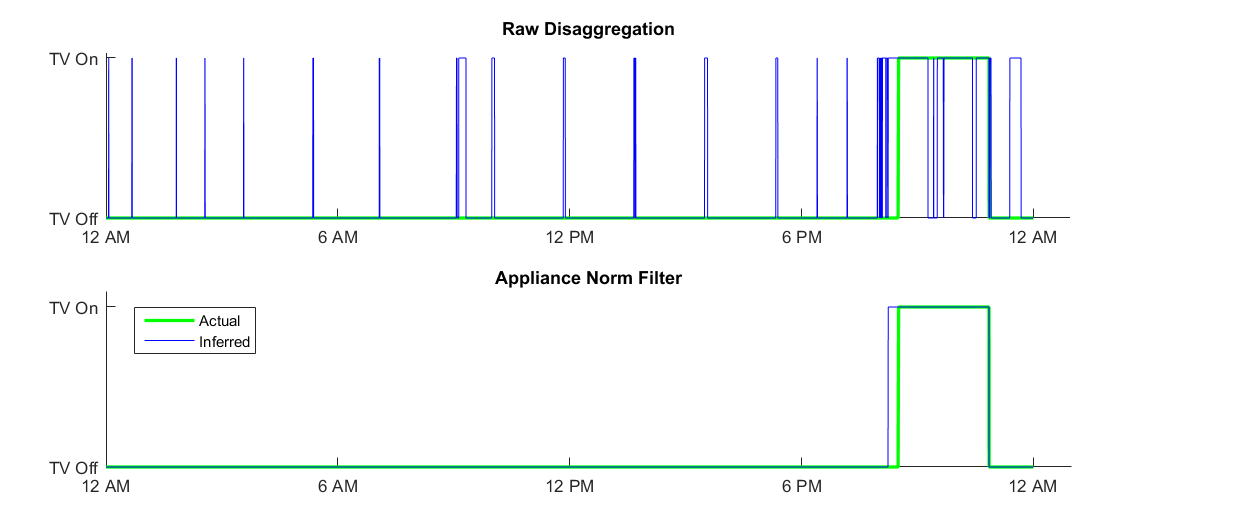
\includegraphics[width=1\textwidth]{billeder/F1vsnormF1.png}}

\put(400,140){F1 $= 0.6656$}
\put(400,130){Accuracy $= 0.5346$}

\put(400,50){F1 $= 0.6866$}
\put(400,40){Accuracy $= 0.5487$}

\end{picture}
\caption{TV event detection}
\label{fig:TVEVENT}
\end{figure}

The "Raw Disaggregation" is before applying a simple norm filter, the second illustration is after the norm filter. The norm filter used is the same as in in Section \ref{sec:NormFilter}. Visually the difference between the two signals is huge. The signal after the norm filter is much better then the signal prior to the norm filter. When looking at the F1 and accuracy scores of the two signals, the norm filter have only improved the signal with approximately 2\%.  

This raises the question: \textit{is the F1 score a good indicator, and how high does the score need to be before it is application ready?} The F1 score seems to be generality adopted due to its simplicity and and acceptance in other areas of binary classification~\citep{RefWorks:35}. The F1 score required for a acceptable application can be dependent on many aspects. During the experiments, applications with a F1 score lower than 0.8 was generality influence much by interference from other devices. Where F1 scores higher than 0.8 could be filtered more easily, and gave more intuitive correct results.  

The conclusion being that a functioning \ab{NILM} solution requires commitment. A successful system will require the metering company to develop, or at least install, a meter capable of high speed data collection or processing. Furthermore must the residents have a interest in helping improving the accuracy, in order to get the best results. This could be done by registering appliances on a smart phone or tablet as suggested by Weiss~\citep{RefWorks:23}.

\section{NILM Privacy Concerns}
As shown in Chapter \ref{sec:CaseStudy} it is possible to gesture about the TV habits of a household. Potentially can the usage pattern for any appliance be derived using \ab{NILM} techniques. Researchers have shown that even the current movie shown on a TV can be deduced by looking at the power profile \citep{RefWorks:39}. With \ab{NILM} techniques it is more or less possible to track the behaviour of a residential household \citep{RefWorks:37}.

This kind of possible surveillance raises some privacy concerns. Some simple techniques can be used to mask the appliances from a NILM applications, to improve privacy. It have been shown that down-sampling the consumption signal makes it harder for the \ab{NILM} algorithms. Quantifying the signal by rounding it to a multiple of a pre-defined quantization factor also helps mask signals. Averaging the consumption signal over a time period is also shown to have a masking effect~\citep{RefWorks:40}. Common for all these techniques is that they must be actively build in the meter and transfer mechanisms to mask the appliance data. This will only be the case if the meter company have the same privacy concerns as the users. 

An other approach is to use \ab{NILL}[non-intrusive load leveling] to mask the appliance signals. \ab{NILL} is a technique where a capacitive device like a battery is used to store energy. This energy is used to camouflage power signatures from the household~\citep{RefWorks:36}. 

\begin{figure}[H]
\centering
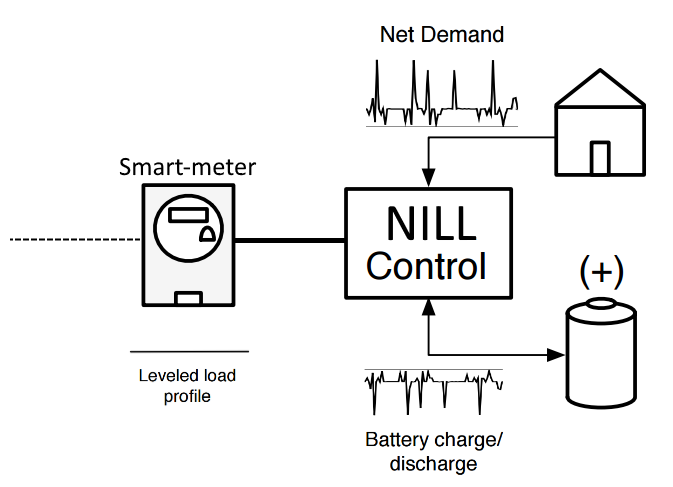
\includegraphics[width=0.5\textwidth]{billeder/NILLILU.png}
\caption{NILL illustration. Inspired by \citep{RefWorks:36}}
\label{fig:NILL}
\end{figure}

This principle is illustrated in figure \ref{fig:NILL}. A NILL solution can be installed after the smart-meter and can provide privacy, without the consent of the electricity utility providers.

At the current state of \ab{NILM} is the technology not accurate enough to make reliable detailed surveillance of the household residents. But still advanced enough to raise some privacy concerns. There are many benefits with advancing the possibilities of NILM. Many services can be developed that can support and help the resident. Some of the possibilities are in saving systems and home automation. This systems could greatly benefit the resident of the household. Electronic companies could also benefit from getting accurate user statistics for there devices. But advancing the technology in this direction would also serve to expose the privacy of the home. This raises the quotations about who are allowed accesses such sensitive information, and for what purposes must it be used. 

% 1 pages
\glsresetall
\chapter{Conclusion}
%----------------------------------------------------------------------------------------
%	REFERENCE LIST
%----------------------------------------------------------------------------------------
\begingroup
	\raggedright
	\bibliography{bibtex/literature}
\endgroup

%----------------------------------------------------------------------------------------
\end{document}